%definira klasu dokumenta 
\documentclass[12pt]{report} 

%prostor izmedu naredbi \documentclass i \begin{document} se zove uvod. U njemu se nalaze naredbe koje se odnose na cijeli dokument

\usepackage[croatian]{babel} 
\usepackage{amssymb}
\usepackage{amsmath}
\usepackage{txfonts}
\usepackage{mathdots}
\usepackage{titlesec}
\usepackage{array}
\usepackage{lastpage}
\usepackage{etoolbox}
\usepackage{tabularray}
\usepackage{color, colortbl}
\usepackage{adjustbox}
\usepackage{geometry}
\usepackage[classicReIm]{kpfonts}
\usepackage{hyperref}
\usepackage{fancyhdr}

\usepackage{float}
\usepackage{setspace}
\usepackage{graphicx}
\restylefloat{table}


\patchcmd{\chapter}{\thispagestyle{plain}}{\thispagestyle{fancy}}{}{} %redefiniranje stila stranice u paketu fancyhdr

%oblik naslova poglavlja
\titleformat{\chapter}{\normalfont\huge\bfseries}{\thechapter.}{20pt}{\Huge}
\titlespacing{\chapter}{0pt}{0pt}{40pt}


\linespread{1.3} %razmak između redaka

\geometry{a4paper, left=1in, top=1in,}  %oblik stranice

\hypersetup{ colorlinks, citecolor=black, filecolor=black, linkcolor=black,	urlcolor=black }   %izgled poveznice


%prored smanjen između redaka u nabrajanjima i popisima
\newenvironment{packed_enum}{
	\begin{enumerate}
		\setlength{\itemsep}{0pt}
		\setlength{\parskip}{0pt}
		\setlength{\parsep}{0pt}
	}{\end{enumerate}}

\newenvironment{packed_item}{
	\begin{itemize}
		\setlength{\itemsep}{0pt}
		\setlength{\parskip}{0pt}
		\setlength{\parsep}{0pt}
	}{\end{itemize}}




%boja za privatni i udaljeni kljuc u tablicama
\definecolor{LightBlue}{rgb}{0.9,0.9,1}
\definecolor{LightGreen}{rgb}{0.9,1,0.9}

%Promjena teksta za dugačke tablice
\DefTblrTemplate{contfoot-text}{normal}{Nastavljeno na idućoj stranici}
\SetTblrTemplate{contfoot-text}{normal}
\DefTblrTemplate{conthead-text}{normal}{(Nastavljeno)}
\SetTblrTemplate{conthead-text}{normal}
\DefTblrTemplate{middlehead,lasthead}{normal}{Nastavljeno od prethodne stranice}
\SetTblrTemplate{middlehead,lasthead}{normal}

%podesavanje zaglavlja i podnožja

\pagestyle{fancy}
\lhead{Programsko inženjerstvo}
\rhead{Ples}
\lfoot{$Program Tvoj Kompjutera$}
\cfoot{stranica \thepage/\pageref{LastPage}}
\rfoot{\today}
\renewcommand{\headrulewidth}{0.2pt}
\renewcommand{\footrulewidth}{0.2pt}


\begin{document} 
	
	
	
	\begin{titlepage}
		\begin{center}
			\vspace*{\stretch{1.0}} %u kombinaciji s ostalim \vspace naredbama definira razmak između redaka teksta
			\LARGE Programsko inženjerstvo\\
			\large Ak. god. 2022./2023.\\
			
			\vspace*{\stretch{3.0}}
			
			\huge {$Ples$}\\
			\Large Dokumentacija, Rev. \textit{$1$}\\
			
			\vspace*{\stretch{12.0}}
			\normalsize
			Grupa: \textit{$ProgramTvogKompjutera$}\\
			Voditelj: \textit{Mateja Golec}\\
			
			
			\vspace*{\stretch{1.0}}
			Datum predaje: \textit{$18$. $11$. $2022$.}\\
	
			\vspace*{\stretch{4.0}}
			
			Nastavnik: \textit{Hrvoje Nuić}\\
		
		\end{center}

	
	\end{titlepage}

	
	\tableofcontents


	\chapter{Dnevnik promjena dokumentacije}
		
		\textbf{\textit{Kontinuirano osvježavanje}}\\
				
		
		\begin{longtblr}[
				label=none
			]{
				width = \textwidth, 
				colspec={|X[2]|X[13]|X[3]|X[3]|}, 
				rowhead = 1
			}
			\hline
			\textbf{Rev.}	& \textbf{Opis promjene/dodatka} & \textbf{Autori} & \textbf{Datum}\\[3pt] \hline
			0.1 & Napravljen predložak.	& Lara Đaković & 30.10.2022. 		\\[3pt] \hline
			0.2 & Dodana 2 \textit{Use Case} dijagrama - admin i vlasnik kluba te opisi za dio obrazaca uporabe& Lara Đaković & 1.11.2022. \\[3pt] \hline 
			0.3 & Dodan opis projektnog zadatka & Nina Đurić & 1.11.2022. \\[3pt] \hline
			0.4 & Dodani funkcionalni zahtjevi & Mateja Golec & 2.11.2022. \\[3pt] \hline 
			0.5 & Dodan \textit{Use Case} dijagram - neregistrirani korisnik, klijent i trener te opisi za dio obrazaca uporabe& Ana Vrabec & 3.11.2022.\\[3pt] \hline 
			0.6 & Dodan UC za neregistriranog korisnika i admina & Lucija Domić & 3.11.2022.\\[3pt] \hline 			
			0.7 & Ispravak obrazaca uporabe i dijagrama obrazaca uporabe za neregistriranog korisnika, klijenta i trenera & Ana Vrabec & 4.11.2022.\\[3pt] \hline 	
			0.8 & Dodan sekvencijski dijagram Prijava trenera i funkcionalnosti & Mateja Golec & 7.11.2022. \\[3pt] \hline
			0.9 & Dodani opisi obrazaca uporabe za klub & Karlo Boroš & 5.11.2022. \\[3pt] \hline
			0.10 & Dodan opis baze podataka i opis tablica Tecaj, Ples, Lokacija, PlesnjakPles i Trening & Lara Đaković & 7.11.2022. \\[3pt] \hline 	
			0.11. & Dodani sekvencijski dijagrami Upravljanje tečajem i Upravljanje plesovima & Nina Đurić & 9.11.2022. \\[3pt] \hline
			0.12 & Dodani ostali zahtjevi & Ana Vrabec & 9.11.2022. \\[3pt] \hline
			0.13 & Dodani opisi tablica za Klub, Korisnik, TrenerPrijava, Plesnjak, KorisnikTecaj & Karlo Boroš & 9.11.2022. \\[3pt] \hline	
			0.14 & Promjena sekvencijskih dijagrama Prijava trenera i Upravljanje tečajem & Mateja Golec & 16.11.2022. \\[3pt] \hline	
			0.15 & Promjenjen opis, popravljeni opisi i tablice baze & Nina Đurić & 16.11.2022. \\[3pt] \hline	
			\textbf{1.0} & Verzija samo s bitnim dijelovima za 1. ciklus & * & 18.11.2022. \\[3pt] \hline 
			
		\end{longtblr}
	
	
		\textit{Moraju postojati glavne revizije dokumenata 1.0 i 2.0 na kraju prvog i drugog ciklusa. Između tih revizija mogu postojati manje revizije već prema tome kako se dokument bude nadopunjavao. Očekuje se da nakon svake značajnije promjene (dodatka, izmjene, uklanjanja dijelova teksta i popratnih grafičkih sadržaja) dokumenta se to zabilježi kao revizija. Npr., revizije unutar prvog ciklusa će imati oznake 0.1, 0.2, …, 0.9, 0.10, 0.11.. sve do konačne revizije prvog ciklusa 1.0. U drugom ciklusu se nastavlja s revizijama 1.1, 1.2, itd.}

	\chapter{Opis projektnog zadatka}
\usepackage{graphicx}

\textbf{\textit{dio 1. revizije}}\\

\textit{Na osnovi projektnog zadatka detaljno opisati korisničke zahtjeve. Što jasnije opisati cilj projektnog zadatka, razraditi problematiku zadatka, dodati nove aspekte problema i potencijalnih rješenja. Očekuje se minimalno 3, a poželjno 4-5 stranica opisa.	Teme koje treba dodatno razraditi u ovom poglavlju su:}
\begin{packed_item}
	\item \textit{potencijalna korist ovog projekta}
	\item \textit{postojeća slična rješenja (istražiti i ukratko opisati razlike u odnosu na zadani zadatak). Dodajte slike koja predočavaju slična rješenja.}
	\item \textit{skup korisnika koji bi mogao biti zainteresiran za ostvareno rješenje.}
	\item \textit{mogućnost prilagodbe rješenja }
	\item \textit{opseg projektnog zadatka}
	\item \textit{moguće nadogradnje projektnog zadatka}
\end{packed_item}

\textit{Za pomoć pogledati reference navedene u poglavlju „Popis literature“, a po potrebi konzultirati sadržaj na internetu koji nudi dobre smjernice u tom pogledu.}
\eject

\section{Opis projektnog zadatka 'Ples'}

\textit{Cilj ovog projekta je razviti programsku podršku za stvaranje web aplikacije “Ples”, koja korisniku olakšava pronalaženje i organizaciju plesnih tečajeva i plesnjaka, time uvelike olakšavajući život ljubiteljima plesa jer će imati sve što im je potrebno u jednoj web aplikaciji. Procjenjeno vrijeme potrebno za izradu projekta je tri mjeseca}

\textit{Neregistriranom korisniku se, otvaranjem stranice, prikazuje karta sa dostupnim plesnjacima i lokacijama klubova. Neregistrirani korisnik također može i pregledati profile klubova i tipove plesova koji nudi, a kako bi si olakšao pretragu, plesnjake može filtrirati po tipu plesa, klubu koji ga organizira i tipovima plesa. Isto tako, klubove je moguće filtrirati po tipovima plesa za koje organiziraju tečajeve. 
	Neregistrirani korisnik može kreirati novi račun za klijenta navođenjem sljedećih obaveznih informacija:
}
\begin{packed_item}
	\item \textit{korisničko ime}
	\item \textit{lozinka}
	\item \textit{ime}
	\item \textit{prezime}
	\item \textit{spol}
	\item \textit{datum rođenja}
	\item \textit{broj mobitela}
	\item \textit{email adresa}
\end{packed_item}

\textit{Korisnik također može, ali i ne mora unijeti sljedeće informacije:}

\begin{packed_item}
	\item \textit{opis plesnog iskustva}
	\item \textit{fotografija}
\end{packed_item}

\textit{Neregistrirani korisnik također može kreirati novi račun za klub, te će mu za isto biti potrebno navođenje sljedećih informacija:}

\begin{packed_item}
	\item \textit{korisničko ime}
	\item \textit{lozinka}
	\item \textit{ime kluba}
	\item \textit{adresa sjedišta}
	\item \textit{broj telefona}
	\item \textit{email}
\end{packed_item}

\textit{Nakon stvaranja novog računa za klub, korisnik mora čekati na potvrdu od strane administratora.  Nakon provedene registracije, korisnik može mijenjati sve informacije potrebne za registraciju po volji. Također, korisnik uvijek može izbrisati svoj račun.}

\textit{Registrirani korisnik može obnašati ulogu klijenta, ulogu kluba, uloge trenera i klijenta ili ulogu administratora.}

\textit{\underbar{Klijentu} se na karti prikažu i tečajevi slobodni za upis. Rezultate može filtrirati po vremenu i tipu plesa. Sličnu mogućnost nalazimo na web stranici \url{https://danceprogram.duke.edu/courses}, gdje korisnici filtriraju tečajeve po vremenu i vrsti tečaja.}

\begin{figure}[H]
	\centering
	\includegraphics[scale=1]{screenshot001}
	\caption{Primjer prikaza tečajeva}
	\label{fig:screenshot001}
\end{figure}

\textit{Nakon što odabere željeni tečaj, klijentu se prikazuju informacije o odabranom tečaju, primjerice, vrsta plesa, kalendar te ime, prezime i slika trenera. Ponovno sličnu mogućnost nalazimo na \url{https://danceprogram.duke.edu/courses/dance-composition}, gdje, kad odaberemo tečaj, prikažu nam se neke informacije o tečaju, u ovom slučaju, vrsta plesa i razdoblje godine u kojem se taj tečaj izvodi, međutim, na ranije spomenutoj web stranici, pri odabiru tečaja, ne nalazimo informacije o treneru i kalendar, što je jedna od odlika projektne aplikacije.}

\begin{figure}[H]
	\centering
	\includegraphics[scale=1]{screenshot002}
	\caption{Primjer prikaza informacija o tečajevu}
	\label{fig:screenshot002}
\end{figure}

\textit{ U kalendaru korisnik može pregledati sve zapisane termine tečaja i njihovu lokaciju s dvoranom. Također, klijent može pregledati i aktivne prijave za tečaj od određenog kluba i prijaviti se na njih.}

\textit{\underbar{Klubovi} organiziraju plesnjake koji se mogu izvoditi i na lokacijama van kluba, a sadrže naziv, opis i sliku. Plesnjaci nisu ograničeni na samo jedan tip plesa, već je moguće plesati više različitih vrsta plesova.}

\textit{Na profilu kluba se nalaze informacije o imenu kluba, broj telefona, kratki opis, poveznica na stranicu s grupama za upis, popis plesova koje njihovi treneri nude, prikaz lokacija na karti te popis dvorana po lokacijama.}

\textit{Plesni Klub Tina, na poveznici \url{https://www.plesniklubtina.hr/}, korisnicima također nudi informacije o imenu kluba, broj telefona, kratki opis i lokaciju, koja, za razliku od projektne aplikacije, nije prikazana na karti. Također, za razliku od projektne aplikacije, 'Tina' korisnicima prikazuje svoj mail i sponzora, dok s druge strane ne nudi poveznicu na stranicu s grupama za upis, popis plesova u svom repertoaru i popis dvorana.}

\begin{figure}[H]
	\centering
	\includegraphics[scale=1]{screenshot003}
	\caption{Primjer opisa kluba}
	\label{fig:screenshot003}
\end{figure}

\textit{Klub može objaviti upise za tečaj s krajnjim rokom za prijavu, te može ograničiti upis u grupu postavljanjem dobne granice ili ograničavanjem upisa na samo jedan spol. Zatim se grupi dodjeljuje trener, skup treninga kroz neko vrijeme, gornja granica broja sudionika, te mnoge informacije koje klijentu mogu pomoći pri odabiru grupe, primjerice težina treninga, posebni uvjeti treniranja i pravila ponašanja. Nakon isteka roka, klub radi selekciju prijavljenih klijenata za grupu. Klub može naknadno mijenjati popis klijenata te uređivati i brisati grupe.}

\textit{Jedna od zadaća kluba je također izbor trenera.}

\textit{Ulogu \underbar{trenera} može dobiti i obnašati bilo koji klijent koji određenom klubu pošalje prijavu, motivacijsko pismo i potvrdu u obliku pdf dokumenta da je sposoban držati tečaj plesa, te ga zatim isti klub i potvrdi. Svaki trener ima podstranicu na kojoj se nalazi popis svih grupa koje trenira, a termine može pronaći u kalendaru. Na stranici \url{https://danceprogram.duke.edu/courses} također nailazimo na podstranice trenera, čiji je sadržaj potpuno drugačiji od sadržaja podstranice trenera projektne aplikacije, primjerice, na projektnoj web aplikaciji ne nailazimo na detaljan opis trenera, njegovog školovanja i kompetencija, te broj za kontakt. Projektna web aplikacija također ne sadrži sliku trenera na njegovoj podstranici.}

\begin{figure}[H]
	\centering
	\includegraphics[scale=1]{screenshot004}
	\caption{Primjer podstranice o treneru}
	\label{fig:screenshot004}
\end{figure}

\textit{Trener, nakon otvaranja tečaja, uz opće informacije, dobije i popis klijenata koji su potvrdili svoj dolazak na tečaj.}

\textit{\underbar{Administrator} ima najveće ovlasti. On ima mogućnost mijenjanja, dodavanja i brisanja plesova. Plesovi sadrže naziv, kratki opis, sliku i link na video primjer dotičnog plesa. Također, administrator može pregledati popis svih klijenata i klubova te istima uređivati korisničke račune.}

\textit{nakon izrade modela stranice nadopunit i dodat nadogradnje i prilagodbe}
		

	\chapter{Specifikacija programske potpore}
		
	\section{Funkcionalni zahtjevi}
			\noindent \textbf{Dionici:}
			
	\begin{packed_enum}
				\item  Neregistrirani korisnik
				\item  Registrirani korisnik 
					\begin{packed_enum}
						
						\item  klijent
						\item  vlasnik kluba
						\item  trener
						\item administrator
				
					\end{packed_enum}

				\item Razvojni tim
				\item Asistenti
										
			\end{packed_enum}
			
			\noindent \textbf{Aktori i njihovi funkcionalni zahtjevi:}
			
			
			\begin{packed_enum}
				\item  \underbar{ Neregistrirani korisnik (inicijator) može:}
				
				\begin{packed_enum}
					\item pregledati na karti dostupne plesnjake i lokacije klubova
					\item odabrati profile klubova (ime kluba, kontakt telefon, email adresu, kratki opis)  i pregledati tipove plesa (naziv, kratki opis, slika i link na video primjer plesa) koje ti klubovi nude
					\item registrirati se, kreirati novi korisnički račun za klijenta za koji su mu potrebni korisničko ime, lozinka, ime, prezime, spol, datum rođenja, broj mobitela, email adresa i opcionalno opis plesnog iskustva i fotografija
					\item kreirati novi korisnički račun za klub za koji su mu potrebni korisničko ime, lozinka, ime kluba, adresa sjedišta, telefon i email čime postaje vlasnik kluba

					
				\end{packed_enum}
			
				\item  \underbar{Klijent (inicijator) može:}
				
				\begin{packed_enum}
					
					\item pregledavati i mijenjati osobne podatke
					\item izbrisati svoj korisnički račun
					\item  pregledati na karti tečajeve slobodne za upis 
					\item odabrati tečaj/grupu i dobiti prikaz relevantnih informacija (vrsta plesa, kalendar s terminima tečaja i lokacijama s dvoranama, ime i prezime te sliku trenera)
					\item poslati prijavu klubu da postane trener koja mora sadržavati motivacijsko pismo i potvrdu u pdf formatu da je osposobljen držati tečaj plesa
					\item pregledati aktivne prijave na tečaj/grupu kluba (informacije o treneru, skupu treninga kroz neko vrijeme, maksimalnom broju sudionika, opis s dodatnim informacijama o težini treninga, uvjetima treniranja i pravilima ponašanja) i prijaviti se

					
				\end{packed_enum}
			
			
				\item  \underbar{Vlasnik kluba (inicijator) može:}
				
				\begin{packed_enum}
					\item organizirati plesnjak uz odgovarajući opis (lokacija, naziv, opis i slika) – lokacija plesnjaka može biti na lokaciji kluba ili izvan nje 
					\item potvrditi klijenta kao trenera
					\item objaviti upise za tečaj/grupu s krajnjim rokom prijave i ograničenjem na dob i spol
					\item odabrati klijente koji se primaju na tečaj/grupu 
					\item naknadno mijenjati popis klijenata
					\item uređivati i brisati tečajeve/grupe
					\item pregledavati i mijenjati osobne podatke
					\item izbrisati svoj korisnički račun 

				\end{packed_enum}
			

			
				\item  \underbar{Trener (inicijator) može:}
				
				\begin{packed_enum}
					
					\item imati podstranicu na kojoj vidi popis tečajeva/grupa koje trenira
					\item vidjeti na kalendaru sve termine tečajeva/grupa koje vodi
					\item vidjeti opće informacije tečaja/grupe za kojeg je zadužen i popis klijenata koji bi trebali biti nazočni na tečaju/grupi

				\end{packed_enum}
			

			
				\item  \underbar{Administrator (inicijator) može:}
				
				\begin{packed_enum}
					
					\item može dodati, mijenjati i brisati plesove
					\item  odobriti prijavu kluba za korištenje aplikacije 
					\item pregledati popis svih klijenata i klubova
					\item uređivati korisničke račune

					
				\end{packed_enum}
			
			
				\item  \underbar{Baza podataka(sudionik) može:}
				
				\begin{packed_enum}
					
					\item pohranjuje sve podatke o korisnicima i njihovim ovlastima
					\item pohranjuje sve podatke o plesnim tečajevima i plesnjacima, njihovim lokacijama i opisima

					
				\end{packed_enum}
			\end{packed_enum}
			
			\eject 
			
			
				
			\subsection{Obrasci uporabe}
				
				\textbf{\textit{dio 1. revizije}}
				
				\subsubsection{Opis obrazaca uporabe}

\noindent \underbar{\textbf{UC1 - Registracija korisnika}}
					\begin{packed_item}
	
						\item \textbf{Glavni sudionik: }Neregistrirani korisnik
						\item  \textbf{Cilj:} Stvoriti korisnički račun za pristup sustavu
						\item  \textbf{Sudionici:} Baza podataka
						\item  \textbf{Opis osnovnog tijeka:						
						}
						
						\item[] \begin{packed_enum}
	
							\item Korisnik odabire opciju za registraciju
							\item Korisnik unosi potrebne korisničke podatke
							\item Korisnik prima obavijest o uspješnoj registraciji
							
						\end{packed_enum}
						
						\item  \textbf{Opis mogućih odstupanja:}
						
						\item[] \begin{packed_item}
	
							\item[4.a] Odabir već zauzetog korisničkog imena i/ili e-maila, unos 
korisničkog podatka u nedozvoljenom formatu ili pružanje 
neispravnog e-maila

							\item[] \begin{packed_enum}
								
								\item Sustav obavještava korisnika o neuspjelom upisu i vraća 
ga na stranicu za registraciju
								\item Korisnik mijenja potrebne podatke te završava unos ili 
odustaje od registracije
																
							\end{packed_enum}
														
						\end{packed_item}
					\end{packed_item}
					
					\noindent \underbar{\textbf{UC2 - Registracija kluba}}
					\begin{packed_item}
	
						\item \textbf{Glavni sudionik: }Neregistrirani korisnik
						\item  \textbf{Cilj:} Stvoriti korisnički račun za klub
						\item  \textbf{Sudionici:} Baza podataka
						\item  \textbf{Opis osnovnog tijeka:						
						}
						
						\item[] \begin{packed_enum}
	
							\item Korisnik odabire opciju za registraciju kluba
							\item Korisnik unosi podatke vezano za klub
							\item Korisnik prima obavijest o uspješnoj registraciji
							
						\end{packed_enum}
						
						\item  \textbf{Opis mogućih odstupanja:}
						
						\item[] \begin{packed_item}
	
							\item[4.a] . Odabir već zauzetog korisničkog imena i/ili e-maila, unos korisničkog podatka u nedozvoljenom formatu ili pružanje neispravnog e-mail

							\item[] \begin{packed_enum}
								
								\item Sustav obavještava korisnika o neuspjelom upisu i vraća ga na stranicu za registraciju
								\item Korisnik mijenja potrebne podatke te završava unos ili 
odustaje od registracije
																
							\end{packed_enum}
														
						\end{packed_item}
					\end{packed_item}
					
					\noindent \underbar{\textbf{UC3 - Pregled klubova}}
					\begin{packed_item}
	
						\item \textbf{Glavni sudionik: }Neregistrirani korisnik
						\item  \textbf{Cilj:} Pregledati sve dostupne klubove
						\item  \textbf{Sudionici:} Baza podataka
						\item  \textbf{Opis osnovnog tijeka:						
						}
						
						\item[] \begin{packed_enum}
	
							\item Karta je prikazana prilikom učitavanja aplikacije
							\item Korisnik na karti odabire klub
							\item Prikazuju se tipovi plesa koje pojedini klub nudi
							\item Klubovi se mogu filtrirati po tipovima plesa za koje organizira 
tečaj
							\item Odabir filtra
							\item Prikazuju se filtrirani plesnjaci
							
						\end{packed_enum}
						
						
					\end{packed_item}
					
					\noindent \underbar{\textbf{UC4 -Pregled plesnjaka}}
					\begin{packed_item}
	
						\item \textbf{Glavni sudionik: }Neregistrirani korisnik
						\item  \textbf{Cilj:} Pregledati dostupne plesnjake
						\item  \textbf{Sudionici:} Baza podataka
						\item  \textbf{Opis osnovnog tijeka:						
						}
						
						\item[] \begin{packed_enum}
	
							\item Korisniku se na karti prikazuju dostupni plesnjaci 
							\item Dostupni plesnjaci se mogu filtrirati po:
							
							\item[] \begin{packed_enum}
								
								\item Tipu plesa
								\item Klubu koji ga organizira
								
							\end{packed_enum}
							
							\item Odabir filtra
							\item Prikazuju se filtrirani plesnjaci
						
						\end{packed_enum}	
						
					\end{packed_item}
					
					\noindent \underbar{\textbf{UC5 -Odabir kluba}}
					\begin{packed_item}
	
						\item \textbf{Glavni sudionik: }Neregistrirani korisnik
						\item  \textbf{Cilj:} Pretraga određenog kluba
						\item  \textbf{Sudionici:} Baza podataka
						\item  \textbf{Opis osnovnog tijeka:						
						}
						
						\item[] \begin{packed_enum}
	
							\item Pretraživanje kluba odvija se upisom osnovnih podataka o klubu  
							\item Prikazuju se podatci za traženi klub
							
						\end{packed_enum}	
						
					\end{packed_item}
					
					\noindent \underbar{\textbf{UC6 -Dodavanje plesa}}
					\begin{packed_item}
	
						\item \textbf{Glavni sudionik: }Administrator
						\item  \textbf{Cilj:} Dodati novi ples
						\item  \textbf{Preduvjet:} : Korisnik je registriran i dodijeljena su mu prava administratora
						\item  \textbf{Sudionici:} Baza podataka
						\item  \textbf{Opis osnovnog tijeka:						
						}
						
						\item[] \begin{packed_enum}
	
							\item Prikazuju se dostupni klubovi
							\item Odabire se klub kojem želi dodati određeni ples
							\item Unose se osnovni podatci o plesu
							\item Dodaje se novi ples u bazu podataka
							\item Ples postaje vidljiv unutar mogućih plesova za određeni klub
							
						\end{packed_enum}	
						
					\end{packed_item}
					
					\noindent \underbar{\textbf{UC7 - Izmjena plesa}}
					\begin{packed_item}
	
						\item \textbf{Glavni sudionik: }Administrator
						\item  \textbf{Cilj:} Izmjena postojećeg plesa
						\item  \textbf{Preduvjet:} : Korisnik je registriran i dodijeljena su mu prava administratora
						\item  \textbf{Sudionici:} Baza podataka
						\item  \textbf{Opis osnovnog tijeka:						
						}
						
						\item[] \begin{packed_enum}
	
							\item Prikazuju se dostupni klubovi 
							\item Administrator odabire klub
							\item Administrator odabire ples kojem želi izmijeniti određene 
podatke

							\item Promjene se upisuju u bazu podataka
							\item Izmijene postaju vidljive za odabrani ples
							
						\end{packed_enum}	
						
					\end{packed_item}
					
					\noindent \underbar{\textbf{UC8 - Brisanje plesa}}
					\begin{packed_item}
	
						\item \textbf{Glavni sudionik: }Administrator
						\item  \textbf{Cilj:} Brisanje postojećeg plesa
						\item  \textbf{Preduvjet:} : Korisnik je registriran i dodijeljena su mu prava administratora
						\item  \textbf{Sudionici:} Baza podataka
						\item  \textbf{Opis osnovnog tijeka:						
						}
						
						\item[] \begin{packed_enum}
	
							\item Prikazuju se dostupni klubovi 
							\item Odabir kluba
							\item Odabir plesa koji se želi obrisati
							\item Odabrani ples se uklanja iz baze podataka
							\item Obrisani ples nije više vidljiv u aplikaciji
							
						\end{packed_enum}	
						
					\end{packed_item}
					
					\noindent \underbar{\textbf{UC9 - Odobrenje prijave kluba}}
					\begin{packed_item}
	
						\item \textbf{Glavni sudionik: }Administrator
						\item  \textbf{Cilj:} Odobrenje prijave kluba za korištenje aplikacije 
						\item  \textbf{Preduvjet:} : Korisnik je registriran i dodijeljena su mu prava administratora
						\item  \textbf{Sudionici:} Baza podataka
						\item  \textbf{Opis osnovnog tijeka:						
						}
						
						\item[] \begin{packed_enum}
	
							\item Prikaz svih klubova koji traže pristup sustavu 
							\item Prijava se može odbiti ili prihvatiti
							\item U slučaju prihvaćanja, podatci za klub se spremaju u bazu podataka
							\item Klub je nakon toga vidljiv u aplikaciji
							
						\end{packed_enum}	
						
					\end{packed_item}
					
					\noindent \underbar{\textbf{UC10 - Pregled korisnika}}
					\begin{packed_item}
	
						\item \textbf{Glavni sudionik: }Administrator
						\item  \textbf{Cilj:} Pregledati registrirane korisnike
						\item  \textbf{Preduvjet:} : Korisnik je registriran i dodijeljena su mu prava administratora
						\item  \textbf{Sudionici:} Baza podataka
						\item  \textbf{Opis osnovnog tijeka:						
						}
						
						\item[] \begin{packed_enum}
	
							\item Administrator odabire opciju pregledavanja korisnika 
							\item Prikaže se lista svih ispravno registriranih korisnika s osobnim podatcima
							
						\end{packed_enum}	
						
					\end{packed_item}
					
					
					\noindent \underbar{\textbf{UC11 - Uređivanje korisničkih računa}}
					\begin{packed_item}
	
						\item \textbf{Glavni sudionik: }Administrator
						\item  \textbf{Cilj:} Uređivanje korisničkih računa
						\item  \textbf{Preduvjet:} : Korisnik je registriran i dodijeljena su mu prava administratora
						\item  \textbf{Sudionici:} Baza podataka
						\item  \textbf{Opis osnovnog tijeka:						
						}
						
						\item[] \begin{packed_enum}
	
							\item Odabir hoće li se urediti korisnički račun kluba ili klijenta 
							\item Odabir određenog korisničkog računa
							\item Prikazuju se podatci koje je moguće izmijeniti za određeni korisnički račun
 							\item Promjene se spremaju u bazu podataka
							
						\end{packed_enum}	
						
					\end{packed_item}					
					
										\noindent \underbar{\textbf{UC12 -Prijava u sustav}}
					\begin{packed_item}
	
						\item \textbf{Glavni sudionik: }Klijent
						\item  \textbf{Cilj:} Dobiti pristup korisničkom sučelju
						\item  \textbf{Sudionici:} Baza podataka
						\item  \textbf{Preduvjet:} Registracija
						\item  \textbf{Opis osnovnog tijeka:						
						}
						
						\item[] \begin{packed_enum}
	
							\item Unos korisničkog imena i lozinke
							\item Potvrda o ispravnosti unesenih podataka
							\item Pristup korisničkim funkcijama
							
						\end{packed_enum}
						
						\item  \textbf{Opis mogućih odstupanja:}
						
						\item[] \begin{packed_item}
	
							\item[2.a] Neispravno korisničko ime/lozinka
							\item[] \begin{packed_enum}
								
								\item Sustav obavještava korisnika o neuspješnoj prijavi i vraća ga na stranicu kao neregistriranog korisnika
																
							\end{packed_enum}
														
						\end{packed_item}
					\end{packed_item}

					\noindent \underbar{\textbf{UC13 -Pregled osobnih podataka}}
					\begin{packed_item}
	
						\item \textbf{Glavni sudionik: }Klijent
						\item  \textbf{Cilj:} Pregledati osobne podatke
						\item  \textbf{Sudionici:} Baza podataka
						\item  \textbf{Opis osnovnog tijeka:}
						
						\item[] \begin{packed_enum}
	
							\item Klijent odabire opciju prikaza osobnih podataka
							\item Aplikacija prikazuje osobne podatke
						\end{packed_enum}
						
					\end{packed_item}

					\noindent \underbar{\textbf{UC14 -Promjena osobnih podataka}}
					\begin{packed_item}
	
						\item \textbf{Glavni sudionik: }Klijent
						\item  \textbf{Cilj:} Promijeniti osobne podatke
						\item  \textbf{Sudionici:} Baza podataka
						\item  \textbf{Opis osnovnog tijeka:}
						
						\item[] \begin{packed_enum}
	
							\item Klijent odabire opciju promjene osobnih podataka
							\item Klijent mijenja svoje osobne podatke
							\item Klijent sprema promjene
							\item Ažuriraju se podatci u bazi podataka
						\end{packed_enum}
						
						\item  \textbf{Opis mogućih odstupanja:}
						
						\item[] \begin{packed_item}
	
							\item[2.a] Klijent promjeni osobne podatke, ali ne odabere opciju spremanja promjena
							\item[] \begin{packed_enum}
								
								\item Sustav obavještava klijenta da nije spremio podatke prije izlaska iz prozora
								
							\end{packed_enum}
							
						\end{packed_item}
					\end{packed_item}

					\noindent \underbar{\textbf{UC15 -Brisanje korisničkog računa}}
					\begin{packed_item}
	
						\item \textbf{Glavni sudionik: }Klijent
						\item  \textbf{Cilj:} Obrisati korisnički račun
						\item  \textbf{Sudionici:} Baza podataka
						\item  \textbf{Opis osnovnog tijeka:}
						
						\item[] \begin{packed_enum}
	
							\item Klijent odabire opciju prikaza osobnih podataka
							\item Otvara se stranica s osobnim podatcima klijenta
							\item Klijent briše račun
							\item Korisnički račun briše se iz baze podataka
							\item Otvara se stranica vidljiva neregistriranom korisniku
						\end{packed_enum}
						
					\end{packed_item}
					
					\noindent \underbar{\textbf{UC16 -Pregled tečajeva na karti slobodnih za upis}}
					\begin{packed_item}
	
						\item \textbf{Glavni sudionik: }Klijent
						\item  \textbf{Cilj:} Pregledati na karti tečajeve slobodne za upis
						\item  \textbf{Sudionici:} Baza podataka
						\item  \textbf{Opis osnovnog tijeka:						
						}
						
						\item[] \begin{packed_enum}
	
							\item Klijent odabire opciju prikaza slobodnih tečajeva na karti
							\item Otvara se stranica s kartom i prikazom tečajeva
							\item Ukoliko želi, klijent filtrira tečajeve prema željenom vremenu i vrsti plesa
						\end{packed_enum}
						
						\item  \textbf{Opis mogućih odstupanja:}
						
						\item[] \begin{packed_item}
	
							\item[2.a] Nema tečajeva slobodnih za upis 
							\item[] \begin{packed_enum}
								
								\item Sustav obavještava korisnika da trenutno nema tečajeva slobodnih za upis (općenito ili za određeno mjesto i/ili vrstu plesa)
																
							\end{packed_enum}
														
						\end{packed_item}
					\end{packed_item}
				
					\noindent \underbar{\textbf{UC17 -Odabir tečaja s karte}}
					\begin{packed_item}
	
						\item \textbf{Glavni sudionik: }Klijent
						\item  \textbf{Cilj:} Odabrati jedan od slobodnih tečajeva
						\item  \textbf{Sudionici:} Baza podataka
						\item  \textbf{Preduvjet:} Postoji slobodno mjesto za upis na tečaj
						\item  \textbf{Opis osnovnog tijeka:						
						}
						
						\item[] \begin{packed_enum}
	
							\item Klijent odabire željeni tečaj na karti
							\item Otvara se stranica s prikazom relevantnih informacija o tečaju
						\end{packed_enum}
					\end{packed_item}
				

					\noindent \underbar{\textbf{UC18 - Organizacija plesnjaka}}
					\begin{packed_item}
	
						\item \textbf{Glavni sudionik: }Vlasnik kluba
						\item  \textbf{Cilj:} Organizacija plesnjaka uz opis
						\item  \textbf{Sudionici:} Baza podataka
						\item  \textbf{Opis osnovnog tijeka:						
						}
						
						\item[] \begin{packed_enum}
	
							\item Vlasnik kluba odabirom pretraživanja dolazi na stranicu za unos novog plesnjaka
							\item Vlasnik kluba putem forme upisuje potrebne podatke o plesnjaku
							\item Vlasnik kluba potvrđuje izradu plesnjaka
							\item Potvrdom odabira podaci se spremaju u bazu podataka
						\end{packed_enum}
					\end{packed_item}

					\noindent \underbar{\textbf{UC19 - Objava upisa za tečaj}}
					\begin{packed_item}
	
						\item \textbf{Glavni sudionik: }Vlasnik kluba
						\item  \textbf{Cilj:} Upis klijenata na tečaj
						\item  \textbf{Sudionici:} Baza podataka
						\item  \textbf{Opis osnovnog tijeka:}
						
						\item[] \begin{packed_enum}
	
							\item Vlasnik kluba na izborniku odabire opciju za objavu novog tečaja
							\item Vlasnik kluba treba unijeti potrebne podatke o tečaju
							\item Potvrdnim odabirom podaci o tečaju se spremaju u bazu podataka i postaju dostupni svima na izbor
						\end{packed_enum}
						
						\item  \textbf{Opis mogućih odstupanja:}
						
						\item[] \begin{packed_item}
	
							\item[2.a] Vlasnik kluba nije ispunio sve podatke
							\item[] \begin{packed_enum}
								
								\item Stranica vraća vlasnika kluba natrag te traži od njega unos svih potrebnih podataka
								
							\end{packed_enum}							
						\end{packed_item}
					\end{packed_item}

					\noindent \underbar{\textbf{UC20 - Odabir klijenata za tečaj}}
					\begin{packed_item}
	
						\item \textbf{Glavni sudionik: }Vlasnik kluba
						\item  \textbf{Cilj:} Popuna kvote za tečaj
						\item  \textbf{Sudionici:} Baza podataka, Klijent
						\item  \textbf{Preduvjet:} Postoje prijave za tečaj
						\item  \textbf{Opis osnovnog tijeka:}
						
						\item[] \begin{packed_enum}
	
							\item Vlasnik kluba dobiva popis klijenata koji su se prijavili na tečaj
							\item Vlasnik kluba bira klijente prema ograničenjima koja su postavili
							\item Klikom na potvrdu odabira lista klijenata za tečaj je završena i sprema se u bazu podataka
						\end{packed_enum}
					\end{packed_item}

					\noindent \underbar{\textbf{UC21 - Mijenjanje popisa klijenata}}
					\begin{packed_item}
	
						\item \textbf{Glavni sudionik: }Vlasnik kluba
						\item  \textbf{Cilj:} Promjena popisa klijenata primljenih na tečaj
						\item  \textbf{Sudionici:} Baza podataka, Klijent
						\item  \textbf{Preduvjet:} Postoji popis odabranih klijenata za tečaj
						\item  \textbf{Opis osnovnog tijeka:}
						
						\item[] \begin{packed_enum}
	
							\item Vlasnik kluba iz baze podataka uzima popis trenutnih klijenata na tečaju
							\item Vlasnik kluba miče klijente sa popisa ili dodaje nove, ovisno o potrebi
							\item Promijenjeni popis sprema se natrag u bazu podataka
						\end{packed_enum}
					\end{packed_item}

					\noindent \underbar{\textbf{UC22 - Uređivanje tečaja}}
					\begin{packed_item}
	
						\item \textbf{Glavni sudionik: }Vlasnik kluba
						\item  \textbf{Cilj:} Promjena uvjeta nekog tečaja
						\item  \textbf{Sudionici:} Baza podataka
						\item  \textbf{Preduvjet:} Tečaj postoji i objavljen je
						\item  \textbf{Opis osnovnog tijeka:}
						
						\item[] \begin{packed_enum}
	
							\item Vlasnik kluba na izborniku odabire promjenu tečaja
							\item Iz baze podataka se dopremaju podaci o tečaju
							\item Vlasnik kluba mijenja prethodno određene karakteristike
							\item Vlasnik kluba sprema podatke nakon što je gotov sa izmjenom
							\item Promijenjene karakteristike se spremaju u bazu podataka
						\end{packed_enum}
						
						\item  \textbf{Opis mogućih odstupanja:}
						
						\item[] \begin{packed_item}
	
							\item[2.a] Vlasnik kluba unio je neispravne podatke
							\item[] \begin{packed_enum}
								
								\item Stranica od njega zahtjeva da unese ispravne podatke
								
							\end{packed_enum}
						\end{packed_item}
					\end{packed_item}

					\noindent \underbar{\textbf{UC23 - Brisanje tečaja}}
					\begin{packed_item}
	
						\item \textbf{Glavni sudionik: }Vlasnik kluba
						\item  \textbf{Cilj:} Obrisati tečaj
						\item  \textbf{Sudionici:} Baza podataka
						\item  \textbf{Preduvjet:} Tečaj postoji
						\item  \textbf{Opis osnovnog tijeka:}
						
						\item[] \begin{packed_enum}
	
							\item Vlasnik kluba odabire opciju brisanja tečaja
							\item Tečaj se briše iz baze podataka i nije više dostupan
						\end{packed_enum}
						
					\end{packed_item}

					
					\noindent \underbar{\textbf{UC24 -Slanje prijave za trenera}}
					\begin{packed_item}
	
						\item \textbf{Glavni sudionik: }Klijent
						\item  \textbf{Cilj:} Klijent šalje prijavu određenom klubu kako bi postao njihov trener
						\item  \textbf{Sudionici:} Baza podataka, klub
						\item  \textbf{Opis osnovnog tijeka:						
						}
						
						\item[] \begin{packed_enum}
	
							\item Klijent odabire određeni klub
							\item Klijent odabire opciju slanja prijave za trenera
							\item Otvara se prozor sa formom za unos osobnih podataka i datoteka – motivacijsko pismo i potvrda o sposobnosti vođenja tečaja
							\item Klijent unosi podatke i potvrđuje slanje
							\item Podaci se pohranjuju u bazu podataka
							\item Klubu se aplikaciji prikazuje nova prijava
						\end{packed_enum}
						
						\item  \textbf{Opis mogućih odstupanja:}
						
						\item[] \begin{packed_item}
	
							\item[4.a] Podaci u formi imaju krivi format ili nisu ispunjena obavezna polja
							\item[] \begin{packed_enum}
								
								\item Aplikacija obavještava klijenta da unese ispravne i obavezne podatke
																
							\end{packed_enum}
														
						\end{packed_item}
					\end{packed_item}
					
					\noindent \underbar{\textbf{UC25 – Potvrda prijave za trenera}}
					\begin{packed_item}
	
						\item \textbf{Glavni sudionik: }Klub
						\item  \textbf{Cilj:} Klijent postaje trener u određenom klubu
						\item  \textbf{Sudionici:} Baza podataka, klijent
						\item  \textbf{Preduvjet:} Klijent poslao prijavu za trenera
						\item  \textbf{Opis osnovnog tijeka:}
						
						\item[] \begin{packed_enum}
	
							\item Klub odabire prijavu od određenog klijenta
							\item Klub potvrđuje prijavu
							\item Klijentu se dodjeljuju ovlasti trenera
							\item Prijava se označava kao obrađena
						\end{packed_enum}
							
						\end{packed_item}
					\end{packed_item}
					
					\noindent \underbar{\textbf{UC26 - Odbijanje prijave za trenera}}
					\begin{packed_item}
	
						\item \textbf{Glavni sudionik: }Klub
						\item  \textbf{Cilj:} Klijentu se odbija poslana prijava za trenera
						\item  \textbf{Sudionici:} Baza podataka, klijent
						\item  \textbf{Preduvjet:} Klijent poslao prijavu za trenera
						\item  \textbf{Opis osnovnog tijeka:}
						
						\item[] \begin{packed_enum}
	
							\item Klub odabire prijavu od određenog klijenta
$>$
							\item Klub odbija određenog klijentaa
							\item Prijava se označava kao obrađena
						\end{packed_enum}
						\end{packed_item}
					\end{packed_item}
					
					\noindent \underbar{\textbf{UC27 – Pregled vođenih tečajeva}}
					\begin{packed_item}
	
						\item \textbf{Glavni sudionik: }Trener
						\item  \textbf{Cilj:} Vidjeti popis tečajeva koje vodi
						\item  \textbf{Sudionici:} Baza podataka
						\item  \textbf{Preduvjet:} Trener vodi tečaj za određeni klub
						\item  \textbf{Opis osnovnog tijeka:}
						
						\item[] \begin{packed_enum}
	
							\item Trener odabire opciju za prikaz svojih tečajeva
							\item Aplikacije prikazuje popis tečajeva koje trener vodi
							\item Trener odabire određeni tečaj
							\item Prikazuje se naziv tečaja sa opisom i nužnim informacijama o tečaju
						\end{packed_enum}
						
						\end{packed_item}
					\end{packed_item}
				
				
					\noindent \underbar{\textbf{UC28 - Pregled kalendara s vođenim terminima}}
					\begin{packed_item}
	
						\item \textbf{Glavni sudionik: }Trener
						\item  \textbf{Cilj:} Vidjeti kalendar s popisom treninga koje vodi određenog dana i sata
						\item  \textbf{Sudionici:} Baza podataka
						\item  \textbf{Opis osnovnog tijeka:}
						
						\item[] \begin{packed_enum}
	
							\item Trener odabire opciju za prikaz svojih vođenih termina
							\item Prikazuje se kalendar s označenim terminima kada vodi tečaj
						\end{packed_enum}
						\end{packed_item}
					\end{packed_item}
					
					\noindent \underbar{\textbf{UC29 - Pregled polaznika }}
					\begin{packed_item}
	
						\item \textbf{Glavni sudionik: }Trener
						\item  \textbf{Cilj:} Vidjeti popis nazočnih sudionika na tečaju
						\item  \textbf{Sudionici:} Baza podataka
						\item  \textbf{Preduvjet:} Trener vodi odabrani tečaj
						\item  \textbf{Opis osnovnog tijeka:}
						
						\item[] \begin{packed_enum}
	
							\item Trener odabire određeni tečaja iz popisa tečajeva
							\item Prikazuje se popis sudionika na tečaju s osnovnim osobnim podacima
						\end{packed_enum}
						
						\end{packed_item}
					\end{packed_item}

					\noindent \underbar{\textbf{UC30 - Pregled aktivnih prijava na tečaj kluba }}
					\begin{packed_item}
	
						\item \textbf{Glavni sudionik: }Klijent
						\item  \textbf{Cilj:} Pregledati aktivne prijave na tečajeve od klubova
						\item  \textbf{Sudionici:} Baza podataka
						\item  \textbf{Preduvjet:} Postoje aktivne prijave na tečajeve
						\item  \textbf{Opis osnovnog tijeka:}
						
						\item[] \begin{packed_enum}
	
							\item Klijent odabire opciju prikaza aktivnih prijava na tečajeve
							\item Prikazuje se stranica koja sadrži relevantne informacije o treninzima
						\end{packed_enum}
						
						\end{packed_item}
					\end{packed_item}

					\noindent \underbar{\textbf{UC31 -Prijava na tečaj kluba }}
					\begin{packed_item}
	
						\item \textbf{Glavni sudionik: }Klijent
						\item  \textbf{Cilj:} Prijaviti se na tečaj kluba
						\item  \textbf{Sudionici:} Baza podataka, klub
						\item  \textbf{Preduvjet:} Postoje aktivne prijave na tečaj
						\item  \textbf{Opis osnovnog tijeka:}
						
						\item[] \begin{packed_enum}
	
							\item Klijent odabire opciju prikaza aktivnih prijava na tečajeve
							\item Prikazuje se stranica koja sadrži relevantne informacije o treninzima
							\item Klijent odabire opciju prijave na tečaj
							\item Klijent potvrđuje svoj odabir
							\item Prijava klijenta sprema se u bazu podataka te na listu prijavljenih kluba
						\end{packed_enum}
						
						\end{packed_item}
					\end{packed_item}
					
					
				\subsubsection{Dijagrami obrazaca uporabe}
				\eject		
				
				\begin{figure}[H]
			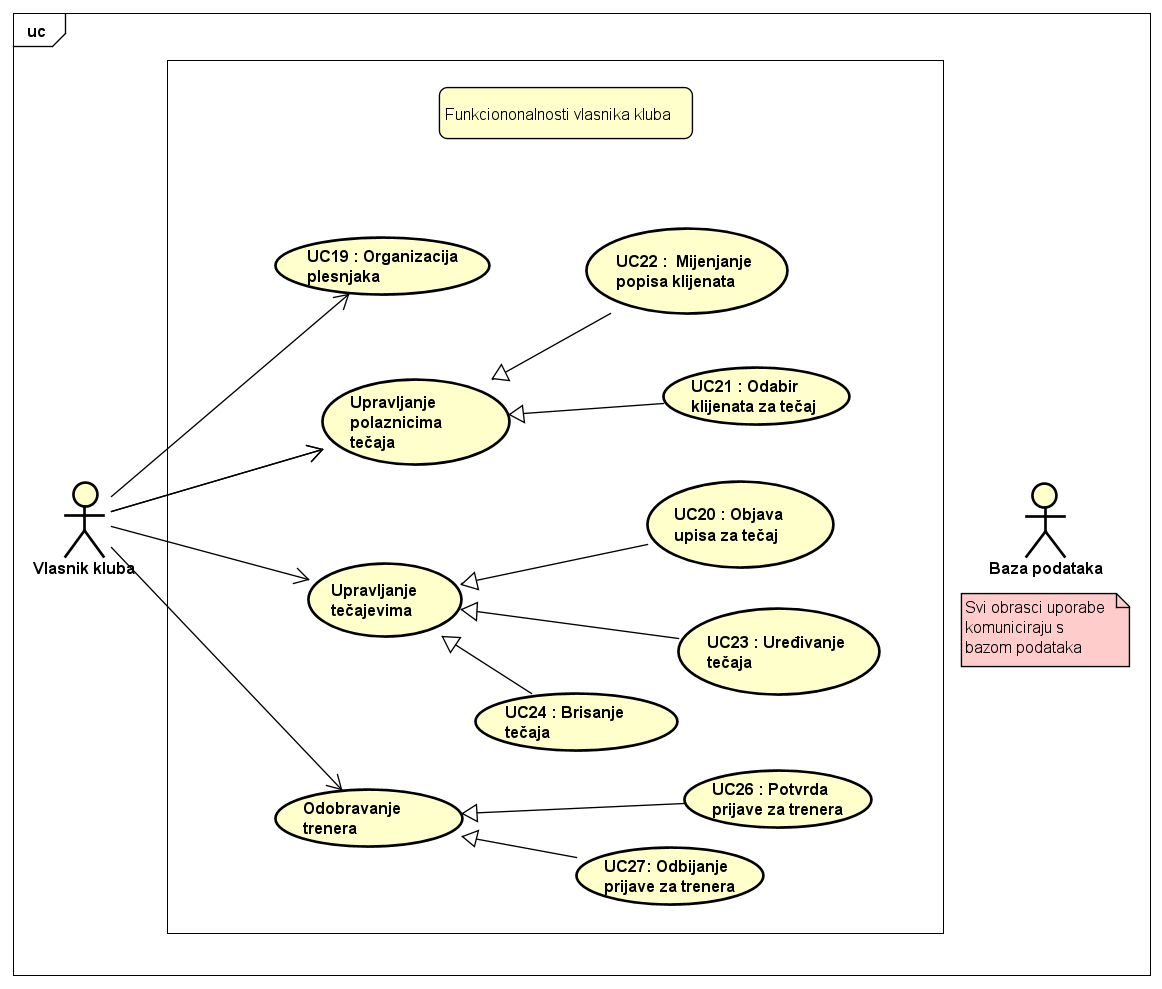
\includegraphics[scale=0.4]{slike/UC_klub.PNG} %veličina u odnosu na širinu linije
			\caption{Dijagram obrasca uporabe, funkcionalnost vlasnika kluba.}
			\label{fig:UC_klub} %label mora biti drugaciji za svaku sliku
		\end{figure}
		
		\begin{figure}[H]
			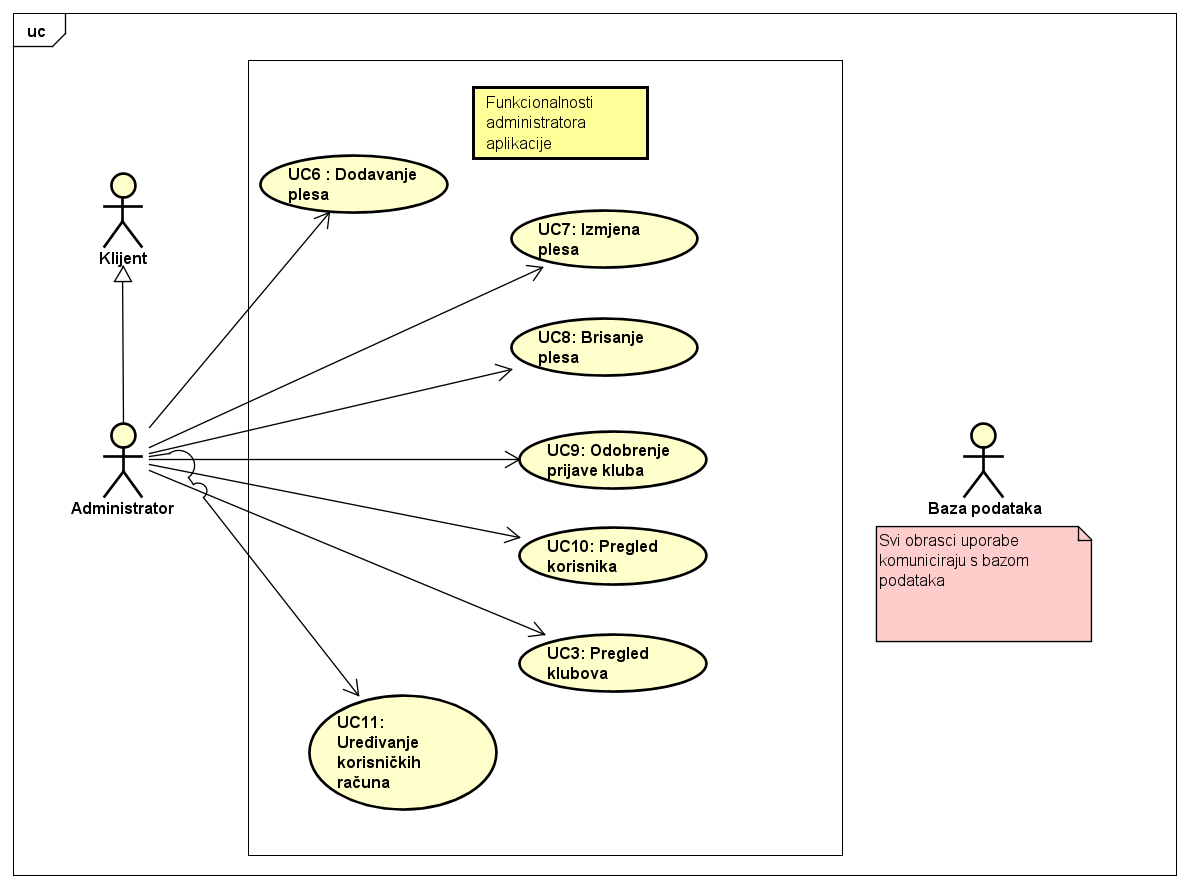
\includegraphics[scale=0.4]{slike/UC_admin.PNG} %veličina u odnosu na širinu linije
			\caption{Dijagram obrasca uporabe, funkcionalnost administratora.}
			\label{fig:UC_admin} %label mora biti drugaciji za svaku sliku
		\end{figure}

		\begin{figure}[H]
			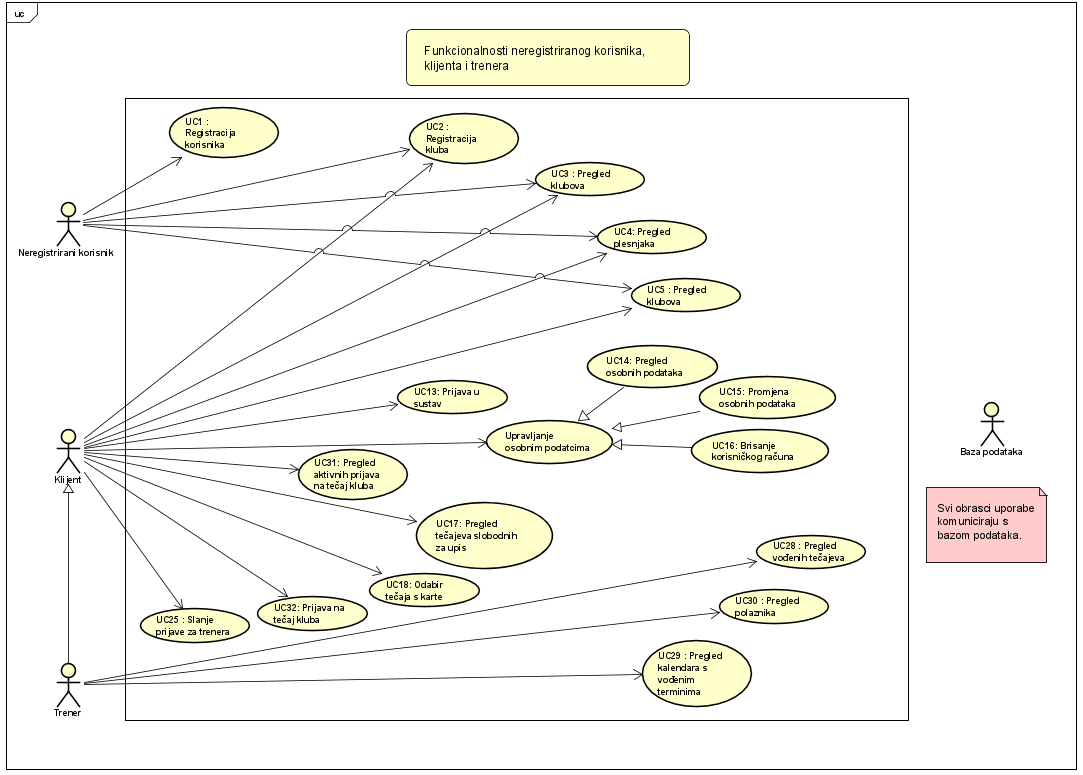
\includegraphics[scale=0.4]{slike/UC_client_trainer_unregistered.PNG} %veličina u odnosu na širinu linije
			\caption{Dijagram obrasca uporabe, funkcionalnost neregistriranog korisnika, klijenta i trenera.}
			\label{fig:UC_klijent_trener_neregistrirani} %label mora biti drugaciji za svaku sliku
		\end{figure}
		
		
				
			\subsection{Sekvencijski dijagrami}
				\noindent \textbf {Obrasci uporabe – UC25, UC26, UC27, UC28, UC29, UC30 - Slanje prijave za trenera, Potvrda prijave za trenera, Odbijanje prijave za trenera, Pregled vođenih tečajeva, Pregled kalendara s vođenim terminima, Pregled polaznika}
Klijent odabire opciju prijave trenera na poslužitelju, a poslužitelj mu vraća formu koju je potrebno ispuniti. Klijent unosi podatke potrebne za prijavu kako bi postao trener, poslužitelj provjerava ispravnost podataka te ih, ako su ispravni, pohranjuje u bazu podataka kao novu prijavu. Vlasnik kluba ima mogućnost pregleda svih prijava za trenere, odabire pregled prijava na poslužitelju, poslužitelj dohvaća podatke iz baze podataka te ih prikazuje vlasniku kluba. Novu prijavu za trenera vlasnik kluba može potvrditi ili odbiti. U slučaju ispunjenih kriterija vlasnik kluba odabire opciju potvrde trenera na poslužitelju, poslužitelj generira objekt novog trenera i unosi podatke o novom treneru u bazu podataka te vraća potvrdu o obavljenim akcijama. Ukoliko kriteriji nisu zadovoljeni, vlasnik kluba odabire opciju odbijanja nove prijave na poslužitelju, poslužitelj mijenja podatke vezane uz tu prijavu u bazi podataka te šalje potvrdu o obavljanju navedenih promjena.  Klijent koji ima potvrđenu ulogu trenera može na poslužitelju zatražiti pregled vođenih tečajeva, poslužitelj dohvaća podatke o njegovim tečajevima iz baze podataka te mu ih prikazuje. Također, može vidjeti prikaz kalendara s terminima tečajeva koje vodi, šalje zahtjev na poslužitelj, poslužitelj dohvaća podatke iz baze podataka, generira kalendar s dohvaćeni podacima te ih prikazuje treneru. Treneru je na poslužitelju omogućen i odabir pregleda popisa klijenata nazočnih na pojedinom terminu, poslužitelj u tom slučaju dohvaća podatke iz baze podataka, generira odgovarajući popis i prikazuje ih treneru. 
				
				%unos slike
		\begin{figure}[H]
			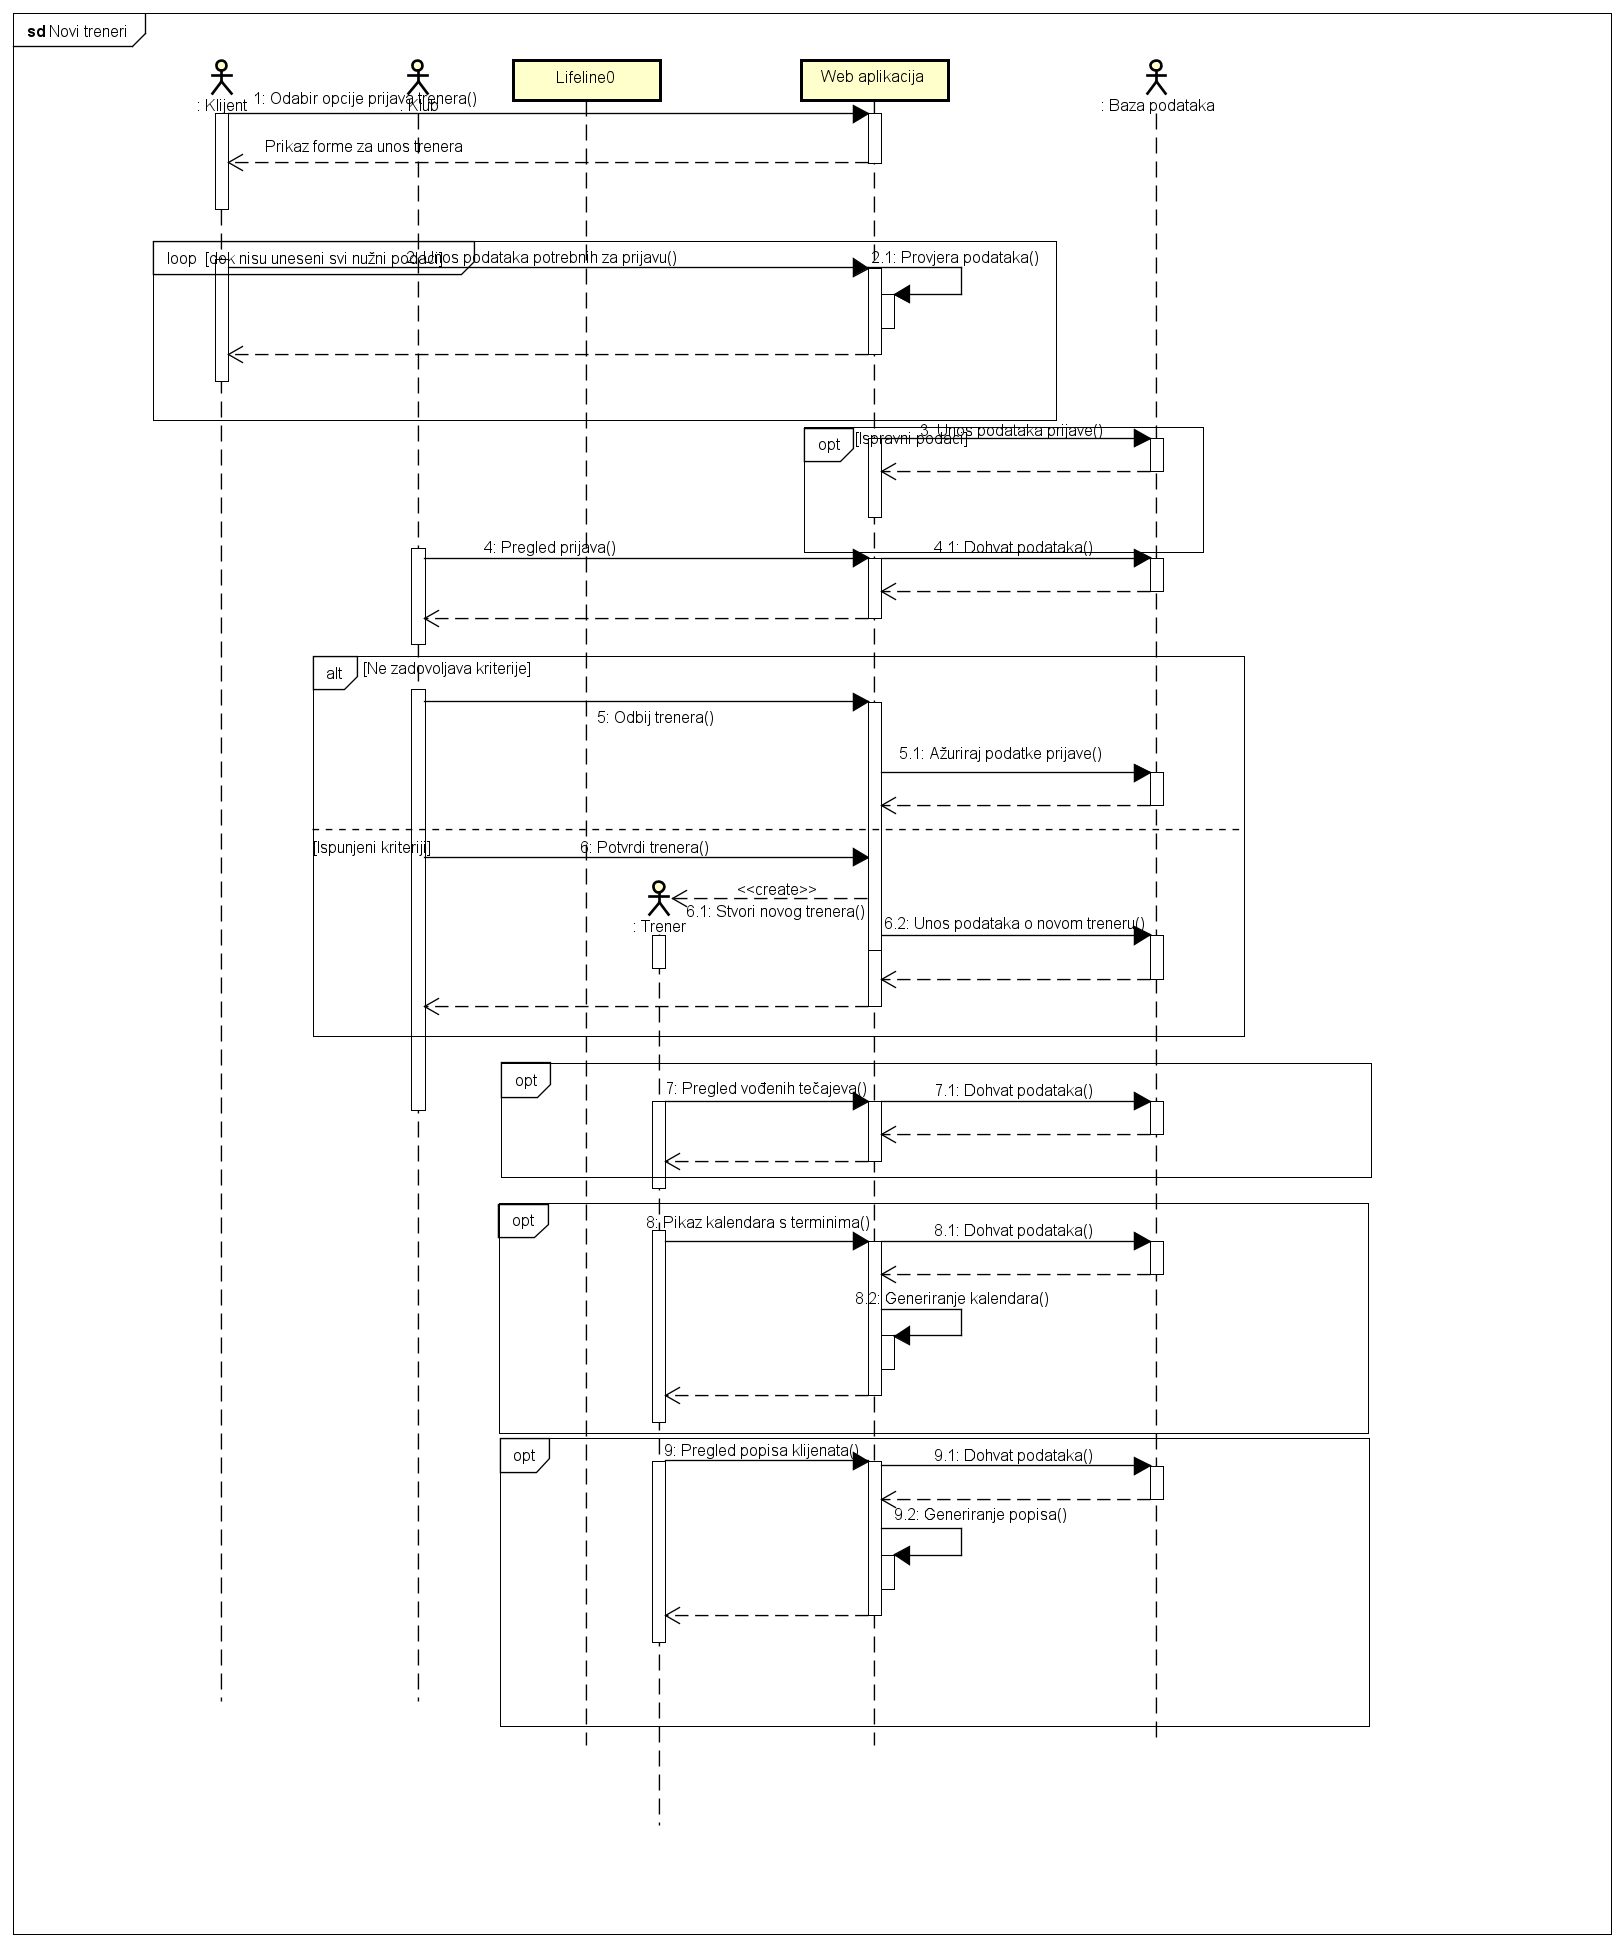
\includegraphics[scale=0.4]{slike/SD-prijavaTrenera.PNG} %veličina slike u odnosu na originalnu datoteku i pozicija slike
			\centering
			\caption{Sekvencijski dijagram - Prijava trenera i njegove funkcionalnosti}
			\label{fig:trener}
		\end{figure}
		
				\noindent \textbf {Obrasci uporabe - UC17, UC20, UC21, UC22, UC32 - Objava upisa na tečaj, pregled tečajeva, prijava na tečaj, odabir klijenata za tečaj i mijenjanje popisa klijenata} 
Vlasnik kluba šalje zahtjev za izradu tečaja, nakon čega mu poslužitelj vraća formu za upis podataka o tečaju. Poslužitelj zatim podatke o tečaju upisuje u bazu. Klijent šalje zahtjev za pregledom tečajeva. Poslužitelj iz baze dohvaća podatke o tečajevima i prikazuje ih klijentu. Klijent odabire jedan tečaj i prijavi se na njega, nakon čega poslužitelj vrši provjeru ispravnosti. Ako je klijent unio ispravne podatke, poslužitelj u bazu unosi podatke o prijavi i vraća korisniku povratnu informaciju o uspješnosti prijave. Vlasnik kluba šalje zahtjev poslužitelju za pregled prijava. Poslužitelj dohvaća prijave iz baze i šalje ih vlasniku kluba na pregled. Vlasnik kluba zatim odlučuje o potencijalnoj potvrdi klijenta na tečaj, nakon čega poslužitelj ažurira status prijave u bazi podataka. Vlasnik kluba po volji može izmijeniti popis klijenata za tečaj, za što prvo mora poslati zahtjev poslužitelju za dohvat podataka o tečaju. Poslužitelj dohvaća podatke iz baze i šalje ih vlasniku kluba. Vlasnik kluba zatim vrši izmjene i potvrđuje ih, nakon čega poslužitelj ažurira podatke o tečaju u bazi.

		\begin{figure}[H]
			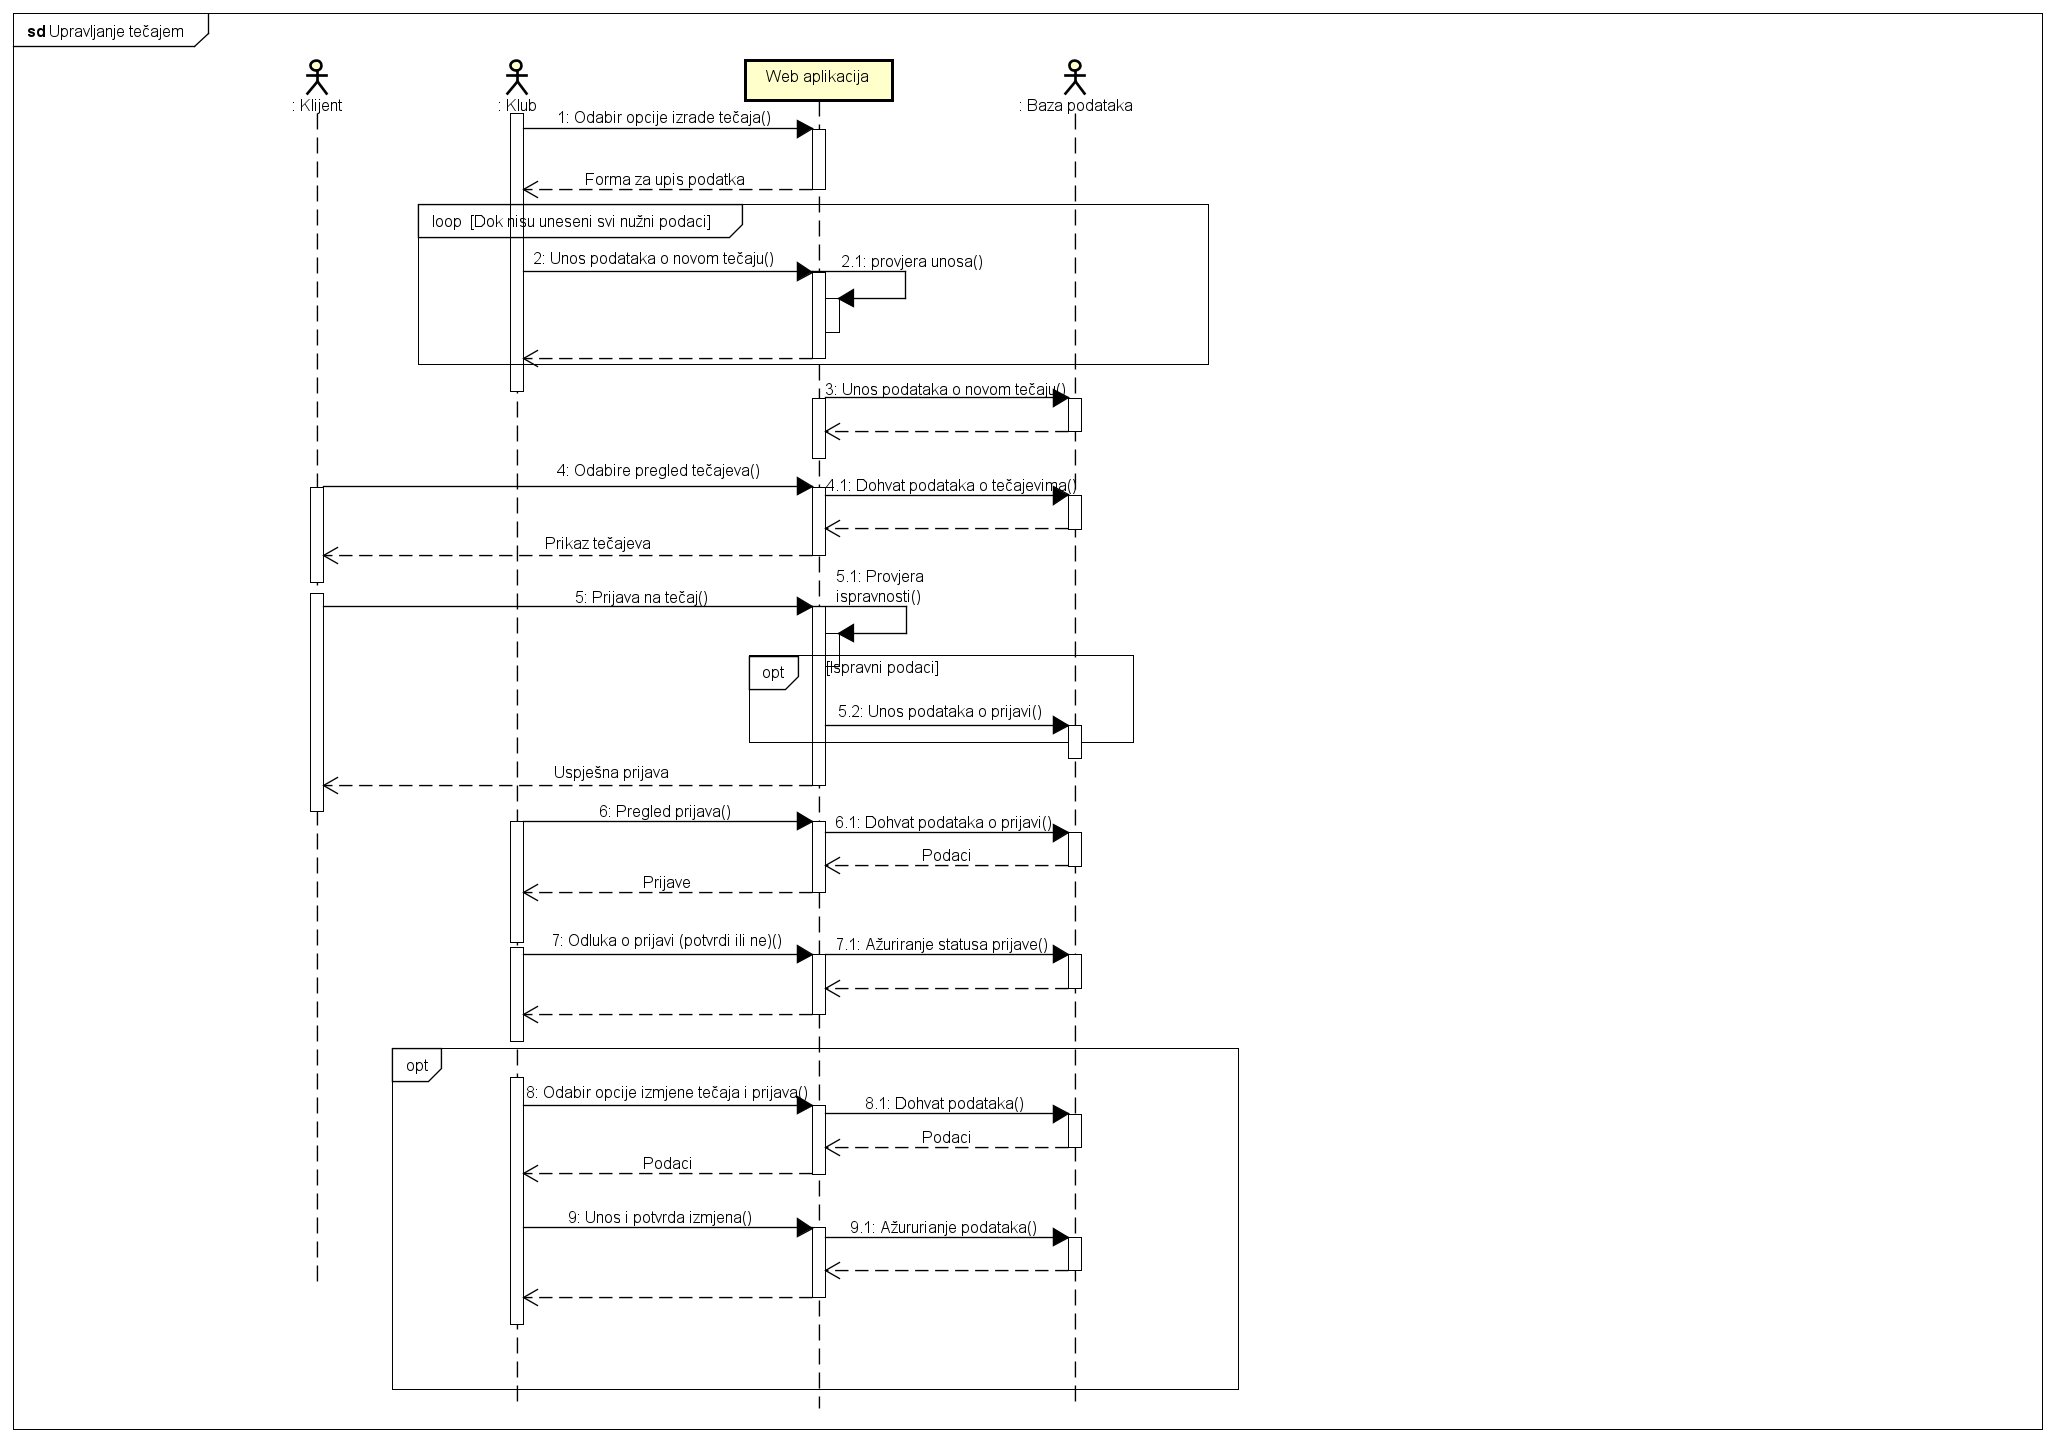
\includegraphics[scale=0.4]{slike/SD-Upravljanje tečajem.PNG} %veličina slike u odnosu na originalnu datoteku i pozicija slike
			\centering
			\caption{Sekvencijski dijagram - Dodavanje tečajeva i prijava na tečajeve}
			\label{fig:tecaj}
		\end{figure}

				\noindent \textbf {Obrasci uporabe UC6, UC7 i UC8 – dodavanje plesova, izmjena plesova i brisanje plesova }
Administrator može dodavati nove plesove i vršiti promjenu nad već postojećim plesovima. Ukoliko se administrator odluči za dodavanje plesa, on šalje poslužitelju zahtjev za stvaranje novog plesa, nakon čega web aplikacija vrši dohvat podataka iz baze te vraća administratoru formu za unos podataka. Administrator ispunjava podatke o novom plesu, a zatim poslužitelj provjerava ispravnost unesenih podataka i šalje ih u bazu podataka. Ukoliko se administrator odluči za izmjenu plesova, on šalje zahtjev poslužitelju za odabir dostupnih plesova. Poslužitelj dohvaća dostupne plesove iz baze te ih vraća poslužitelju. Poslužitelj zatim nad dostupnim plesovima vrši promjene ili briše ples, nakon čega poslužitelj pohranjuje izmjene u bazu podataka
		
		\begin{figure}[H]
			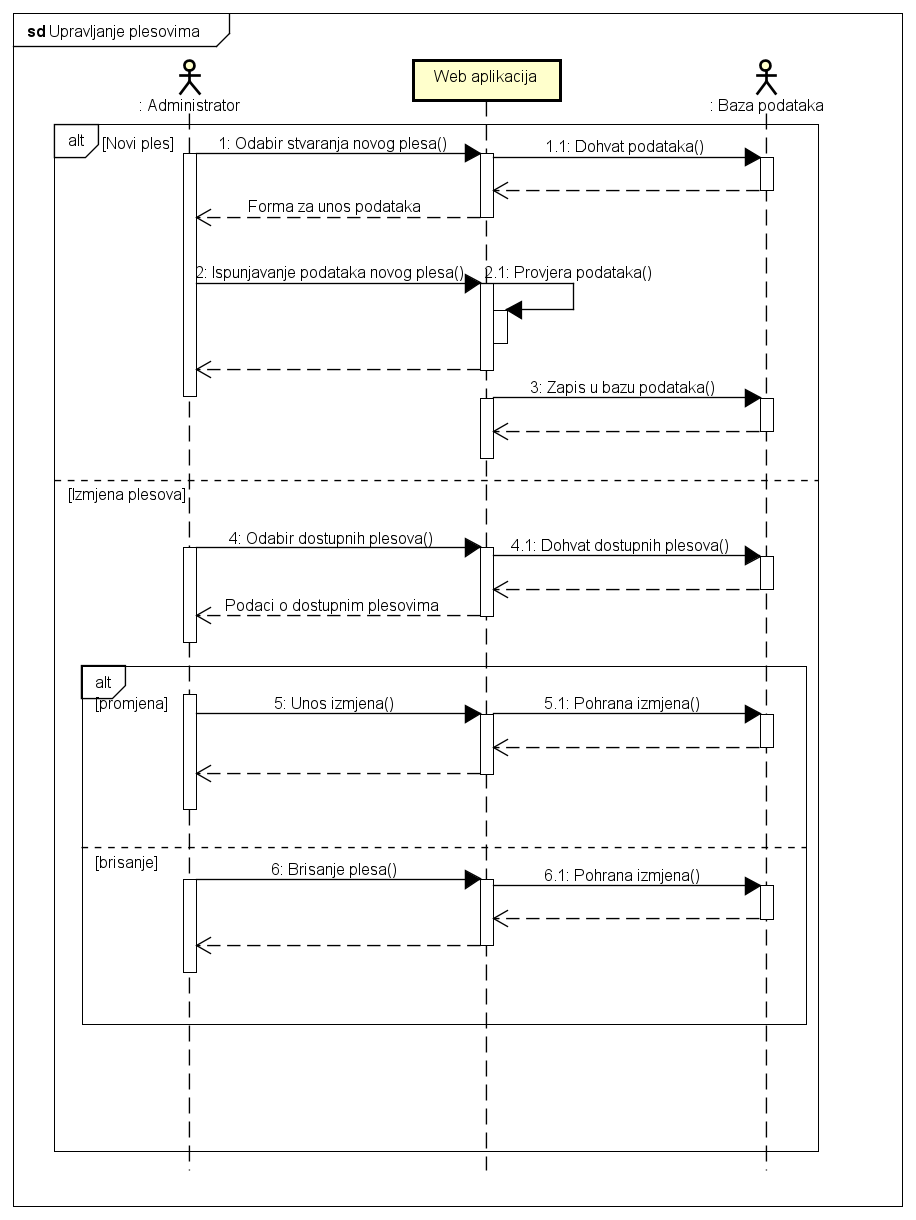
\includegraphics[scale=0.4]{slike/SD-Upravljanje plesovima.PNG} %veličina slike u odnosu na originalnu datoteku i pozicija slike
			\centering
			\caption{Sekvencijski dijagram - Dodavanje, izmjena i brisanje plesova}
			\label{fig:administr}
		\end{figure}
		

				\eject
	
		\section{Ostali zahtjevi}
	
			\begin{packed_item}
	
				\item Sustav treba omogućiti rad više korisnika u stvarnom vremenu
				\item Sustav treba ispravno funkcionirati u svim web preglednicima
				\item Korisničko sučelje i sustav moraju podržavati hrvatsku abecedu (dijakritičke znakove) pri unosu i prikazu tekstualnog sadržaja
				\item Potpuno učitavanje početne stranice aplikacije ne smije trajati duže od 3 sekunde
				\item Izvršavanje dijela programa u kojem se pristupa bazi podataka ne smije trajati duže od 4 sekunde
				\item Sustav treba biti implementiran kao web aplikacija koristeći objektno-orijentirane jezike
				\item Neispravno korištenje korisničkog sučelja ne smije narušiti funkcionalnost i rad sustava
				\item Sustav treba biti jednostavan za korištenje, jasan korisnicima s manje informatičkog iskustva bez opširnih uputa
				\item Nadogradnja sustava ne smije narušavati postojeće funkcionalnosti sustava
				\item Veza s bazom podataka mora biti kvalitetno zaštićena, brza i otporna na vanjske greške
				\item Sustav ne smije omogućiti registraciju korisnika dok nije unesena jaka lozinka (barem jedno veliko slovo, znamenka i specijalni znak)
				\item Sustav koristi srednjoeuropsko standardno vrijeme, GMT+1 
				\item Pristup sustavu mora biti omogućen iz javne mreže pomoću HTTPS
			\end{packed_item}
			 
			 
			 
	
	\chapter{Arhitektura i dizajn sustava}

	\begin{itemize}
		\item \textbf{Proces odabira arhitekture}

Razmatrajući cilj projektnog zadatka, koji je izrada web aplikacije koja olakšava pronalaženje i organizaciju plesnih tečajeva i plesnjaka, specifikacijom svih dionika i njihovih mogućnosti prilikom korištenja aplikacije te definiranjem funkcionalnih zahtjeva zaključili smo da naša aplikacija mora imati tri osnovne razine – \underbar{razinu klijenta, razinu web-aplikacije te razinu baze podataka.} Također, prateća tri sloja koja odgovaraju navedenoj podjeli – \underbar{sloj korisničkog}
\underbar{sučelja, sloj aplikacijske logike te sloj pristupa podacima.} 

Nadalje, slijedeći principe dobrog oblikovanja, kako bi povećali koheziju i smanjili nepotrebne međuovisnosti, kod koji obavlja pojedinu operaciju vezanu uz određeni entitet je grupiran, dok se sve ostalo što nije izravno vezano uz tu funkcionalnost stavlja izvan te operacije. 

Razine također trebaju formirati hijerarhiju, tako da su svi resursi za pristup skupu povezanih usluga na jednom mjestu, čime se omogućuje da viša razina može putem programskog sučelja pristupiti nižoj. 

Također, kako bi si olakšali snalaženje cilj je grupirati sve dijelove programa koji pristupaju ili mijenjaju određene podatke te grupirati procedure koje se izvode slijedno i izmjenjuju podatke. Pomoćne programe primjenjive na više različitih grupa, koji se logički ne mogu smjestiti u ostale grupe odvajamo u grupu pomoćnih programa (utils/shared/common).

Ovisnosti između pojedinih modula želimo smanjiti kako nam neke jednostavnije izmjene ne bi zahtijevale promjene na velikom broju ostalih modula te želimo da nam se jasno vidi povezanost određenih entiteta i njihovih odgovarajućih sučelja. 

U aplikaciji također želimo ostvariti povećanje ponovne uporabivosti što ćemo postići korištenjem programskih knjižnica i radnih okvira. 

Nakon svih razmatranja odabrali smo višeslojnu arhitekturu temeljenu na odnosu klijent-poslužitelj, najsličniju MVC stilu arhitekture.


		\item  \textbf{Višeslojna arhitektura}

Karakteristika klijent-poslužitelj opisuje odnos programa koji surađuju u aplikaciji. Ovaj model arhitekture uključuje razmatranje funkcioniranja klijenta i poslužitelja prije, tijekom i po završetku zajedničke komunikacije.


Aplikacija ima tri osnovna sloja:

1.\textit{Klijentsku komponentu} – sloj s korisničkim sučeljem

2.\textit{Poslužiteljsku komponentu} – sloj aplikacijske logike s implementacijom poslovnih procesa i izračuna

3.\textit{Bazu podataka} – podatkovni sloj za pohranu podataka


\underbar{Klijentska komponenta} predstavljena je web preglednikom, programom koji klijentu omogućuje pregled web-stranica i multimedijskih sadržaja vezanih uz te stranice odnosno ima mogućnost pristupa informacijama i zahtijevanja usluga poslužitelja. Web preglednik je prevoditelj koji web stranicu pisanu u kodu interpretira i prikazuje u klijentu razumljivom obliku. Koristeći web preglednik klijent šalje zahtjeve web poslužitelju.

\underbar{Poslužiteljska komponenta} predstavlja web poslužitelj, program čija je osnovni zadatak pohrana, obrada i dostava web stranica klijentu te nam ona predstavlja centar za razmjenu informacija i pružanje usluga. Komunikacija se odvija na aplikacijskoj razini OSI modela koristeći HTTP protokol prijenosa informacija na webu temeljen na izmjeni poruka zahtjev-odgovor. Sam poslužitelj pokreće web aplikaciju i prosljeđuje joj klijentske zahtjeve. 

Web aplikacija obrađuje klijentske zahtjeve pri čemu prema potrebi pristupa bazi podataka te preko poslužitelja, klijentu vraća odgovor vidljiv u web pregledniku.

Prednosti odabrane arhitekture su te što se slojevi mogu oblikovati odvojeno te sve komponente mogu biti jednostavnije i razumljivije, ostvaruje se podjela brige(separation of concerns) time što svaki sloj brine o svojoj funkcionalnosti i ne miješa se u brige nekog drugog sloja, a njihova međuovisnost ostvaruje se komunikacijom putem sučelja čija se implementacija može prilagoditi u određenom sloju.

Za izradu aplikacije kao radni okvir na klijentskoj strani odabrali smo Vue.js zasnovan na JavaScriptu koji pruža učinkoviti razvoj klijentskog sučelja koristeći već dostupne web komponente. 

Za radni okvir na poslužiteljskoj strani odabrali smo radni okvir Node.js Express koji pruža funkcionalnosti posredniče arhitekture (middleware) i usmjeravanja te Sequlize koji apstrahira pristup bazi podataka i omogućuje jednostavnije kreiranje upita bez obzira koja se baza koristi.

Članovi tima kod pišu u razvojnom okruženju Visual Studio Code, no to razvojno okruženje nije nužno i može se koristiti bilo kojim drugim uređivačem teksta. Jednostavno pokretanje, konfiguraciju i puštanje u pogon te neovisnost o računalu na kojem se kod izvršava omogućava korištenje platforme Docker. Kroz 3 Docker kontejnera pokriveni su svi ključni djelovi/slojevi aplikacije - klijent, poslužitelj i baza podataka te su osigurane točne verzije svih vanjskih biblioteka i alata.

%unos slike
		\begin{figure}[H]
			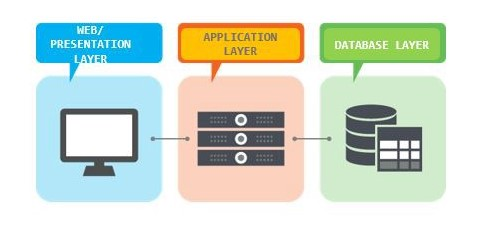
\includegraphics[scale=0.6]{slike/slojevi.jpeg} %veličina slike u odnosu na originalnu datoteku i pozicija slike
			\centering
			\caption{Slojevi arhitehkture}
			\label{fig:sa}
		\end{figure}


		\item \textbf{MVC stil arhitekture}

Arhitektura je  detaljnije razrađena najsličnija stilu arhitekture MVC (Model-View-Controller).

Osnovna karakteristika ovog stila je nezavisan razvoj pojedinih dijelova aplikacije što omogućuje jednostavnije testiranje i razvijanje dijelova sustava te njihove dorade. Korisničko sučelje je odvojeno od ostatka sustava,  a kohezija elemenata se postiže kroz tri sloja, jednog sloja na klijentskoj strani - pogled (View) te dva na poslužiteljskoj strani – nadglednik (Controller) i model (Model).

1.\textit{Model} – predstavlja glavnu komponentu sustava koja sadrži dinamičke strukture podataka odnosno razrede koji opisuju domenu primjene te sadrže pravila i aplikacijsku logiku. Blisko je povezan s bazom podataka aplikacije.

2.\textit{Pogled (View)} – komponenta koja sadrži niz drugih komponente koje služe za prikaz podataka modela i interakciju s korisnikom kroz grafičko sučelje.

3.\textit{Nadglednik (Controller)}  – komponenta koja upravljaja korisničkim zahtjevima prema modelu i odgovorima modela natrag prema pogledima. Omogućuje poveznicu korisničke strane s poslužiteljskom.

%unos slike
		\begin{figure}[H]
			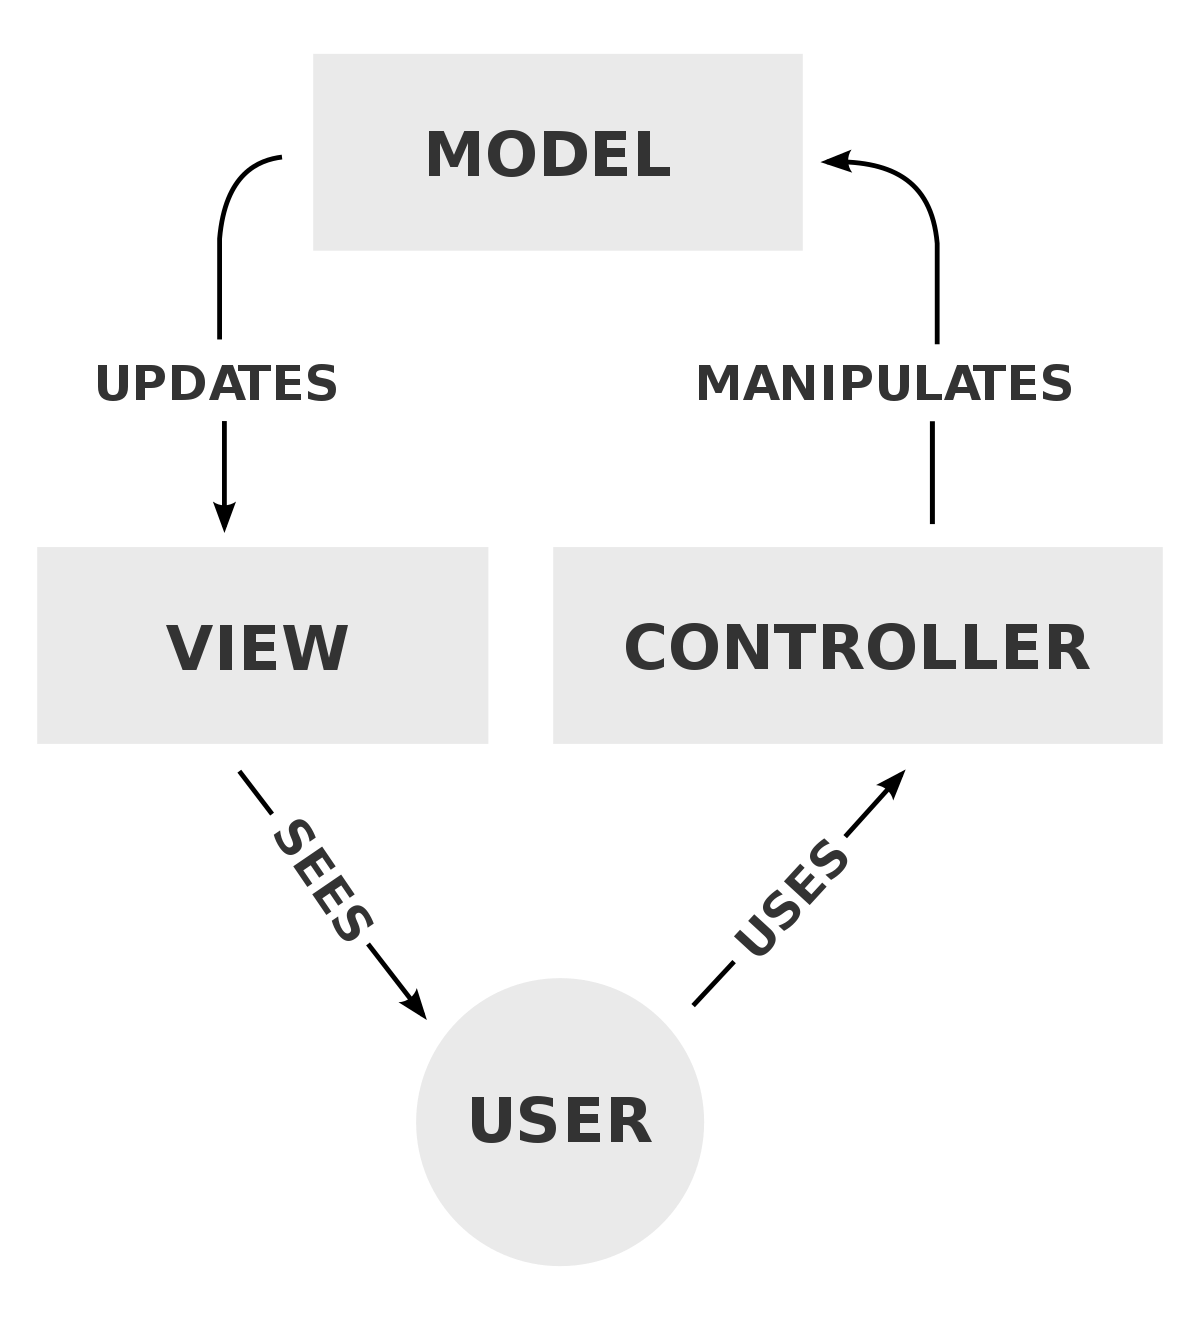
\includegraphics[scale=0.1]{slike/mvc.PNG} %veličina slike u odnosu na originalnu datoteku i pozicija slike
			\centering
			\caption{MVC stil arhitekture}
			\label{fig:mvc}
		\end{figure}
	

	\end{itemize}

	
		

		

				
		\section{Baza podataka}
			
		\textit{
		Za potrebe našeg sustava koristit ćemo relacijsku bazu podataka koja je jednostavna za modeliranje naših potreba - upravljanje podacima o klubovima koji organiziraju određene događaje i korisnicima koji ih pohađaju. Sastavni elementi baze su relacije, odnosno tablice koje sadrže svoje atribute. Zadaća baze podataka je jednostavna pohrana,umetanje, izmjena i dohvat podataka za daljnju obradu. Baza podataka ove aplikacije sastoji se od sljedećih tablica:
			\begin{packed_item}
			
			\item  User
			\item  Club
			\item  Course
			\item  UserCourse
			\item  TrainerAplication
			\item  Event
			\item  Dance
			\item  Location
			\item  EventDance
			\item  Lesson
			
			\end{packed_item}
		}
		
			\subsection{Opis tablica}
				\textit{\textbf{User}} Ovaj entitet opisuje korisnike i sadrži sve informacije o njima. Povezan je sa vezom \textit{One-to-Many} sa TrainerAplication preko \textit{trainerId}, \textit{One-to-Many} sa UserCourse preko \textit{userId} i \textit{One-to-Many} sa Club preko \textit{ownerId}.
				\begin{longtblr}[
					label=none,
					entry=none
					]{
						width = \textwidth,
						colspec={|X[6,l]|X[6, l]|X[20, l]|}, 
						rowhead = 1,
					} %definicija širine tablice, širine stupaca, poravnanje i broja redaka naslova tablice
					\hline \multicolumn{3}{|c|}{\textbf{User}}	    \\ \hline[3pt]
					\SetCell{LightGreen} id & int	& jedinstveni identifikator korisnika \\ \hline
					username & varchar & jedinstveno korisničko ime korisnika\\ \hline 
					firstName & varchar & ime korisnika \\ \hline 
					lastName & varchar & prezime korisnika \\ \hline 
					password & varchar & zaporka za prijavu korisnika \\ \hline 
					gender & enum & spol korisnika \\ \hline 
					dateOfBirth & date & datum rođenja korisnika \\ \hline 
					phone & varchar & jedinstveni kontakt broj korisnika \\ \hline 
					email & varchar & jedinstvena email adresa korisnika \\ \hline 
					role & enum & uloga korisnika \\ \hline
					experienceDescription & varchar & opis korisnikovog iskustva u različitim plesovima \\ \hline 
					image & varchar & fotografija korisnika \\ \hline 
					refreshToken & varchar & korisnikov refresh token \\ \hline 
				\end{longtblr}

				\textit{\textbf{Club}} Ovaj entitet opisuje klubove i sadrži sve informacije o njima. Povezan je sa vezom \textit{One-to-Many} sa TrainerApplocation preko \textit{id}, \textit{One-to-Many} sa Event preko \textit{id}, {One-to-Many} sa Course preko \textit{id}, \textit{Many-to-One} sa User preko \textit{ownerId}, \textit{Many-to-One} sa Location preko \textit{locationId}.
				\begin{longtblr}[
					label=none,
					entry=none
					]{
						width = \textwidth,
						colspec={|X[6,l]|X[6, l]|X[20, l]|}, 
						rowhead = 1,
					} %definicija širine tablice, širine stupaca, poravnanje i broja redaka naslova tablice
					\hline \multicolumn{3}{|c|}{\textbf{Club}}	 \\ \hline[3pt]
					\SetCell{LightGreen} id & int & jedinstveni identifikator treninga \\ \hline
					\SetCell{LightBlue} ownerId & int & identifikator korsnika [ref: $>$ korisnik.id]\\ \hline 
					name & varchar & ime kluba \\ \hline 
					phone & varchar & kontakt broj kluba \\ \hline 
					email & varchar & kontakt mail kluba \\ \hline 
					description & varchar & opis kluba \\ \hline 
					approvalStatus & enum & status odobrenja kluba\\ \hline 
					locationId & int & identifikator lokacije\\ \hline 
				\end{longtblr}

				\textit{\textbf{Course}} Ovaj entitet opisuje tečajeve i sadrži sve informacije o njima. Povezan je sa vezom \textit{Many-to-One} sa User preko \textit{trainerId},  {Many-to-One} sa Club preko \textit{clubId}, {Many-to-One} sa Location preko \textit{locationId}, {Many-to-One} sa Dance preko \textit{danceId}, \textit{One-to-Many} sa UserCourse preko \textit{courseId} i \textit{One-to-Many} sa Lesson preko \textit{id}.
				\begin{longtblr}[
					label=none,
					entry=none
					]{
						width = \textwidth,
						colspec={|X[6,l]|X[6, l]|X[20, l]|}, 
						rowhead = 1,
					} %definicija širine tablice, širine stupaca, poravnanje i broja redaka naslova tablice
					\hline \multicolumn{3}{|c|}{\textbf{Course}}	 \\ \hline[3pt]
					\SetCell{LightGreen} id & int	&  	jedinstveni identifikator tečaja\\ \hline
					\SetCell{LightBlue} locationId	& int & identifikator lokacije [ref: $>$ Lokacija.id]\\ \hline 
					\SetCell{LightBlue} trainerId	& int & identifikator klijenta(trenera) [ref: $>$ Korisnik.id]\\ \hline 		
					name	& varchar &   ime tečaja	\\ \hline 
					description & varchar & opis tečaja  \\ \hline 
					image	& varchar &   url slike za opis tečaja	\\ \hline 
					capacity & int &  kapacitet polaznika \\ \hline 
					minAge	& int &   ograničenje za minimalni broj godina polaznika	\\ \hline 
					maxAge & int &  ograničenje za maksimalni broj godina \\ \hline 
					gender & enum &  ograničenje za spol polaznika 	\\ \hline
					applicationDeadline & datetime & datum za krajnji rok prijave  \\ \hline 
  					maxApplicants & int &  maksimalan broj polaznika \\ \hline 
  					additionalRules & varchar & dodatne informacije i pravila za tečaj  \\ \hline 
  					\SetCell{LightBlue} clubId & int  &  identifikator kluba koji organizira tečaj [ref: $>$ Klub.id]\\ \hline 
  					\SetCell{LightBlue} danceId & int  &   identifikator plesa koji će se plesati na tečaju [ref: $>$ Ples.id]\\ \hline 
					
				\end{longtblr}
				
				\textit{\textbf{UserCourse}} Ovaj entitet opisuje korisnike tečaja i sadrži sve potrebne informacije i reference o njima. Povezan je sa vezom \textit{Many-to-One} sa User preko \textit{userId} i \textit{Many-to-One} sa Course preko \textit{courseId}.
				\begin{longtblr}[
					label=none,
					entry=none
					]{
						width = \textwidth,
						colspec={|X[6,l]|X[6, l]|X[20, l]|}, 
						rowhead = 1,
					} %definicija širine tablice, širine stupaca, poravnanje i broja redaka naslova tablice
					\hline \multicolumn{3}{|c|}{\textbf{UserCourse}}	 \\ \hline[3pt]
					\SetCell{LightGreen} id & int	& jedinstveni identifikator  \\ \hline
					\SetCell{LightBlue} userId	& int & identifikator korisnika [ref: $>$ Korisnik.id]\\ \hline 
					\SetCell{LightBlue} courseId	& int & identifikator tečaja[ref: $>$ Tecaj.id]\\ \hline 
					status & enum & status je li korisnik primljen na tečaj \\ \hline 
				\end{longtblr}

				\textit{\textbf{TrainerApplication}} Ovaj entitet opisuje korisnike koji su se prijavili za trenera i sadrži potrebne informacije o njima. Povezan je sa vezom \textit{Many-to-One} sa User preko \textit{trainerId} i  \textit{Many-to-One} sa Club preko \textit{clubId}.
				\begin{longtblr}[
					label=none,
					entry=none
					]{
						width = \textwidth,
						colspec={|X[6,l]|X[6, l]|X[20, l]|}, 
						rowhead = 1,
					} %definicija širine tablice, širine stupaca, poravnanje i broja redaka naslova tablice
					\hline \multicolumn{3}{|c|}{\textbf{TrainerApplication}}	 \\ \hline[3pt]
					\SetCell{LightGreen} id & int	& jedinstveni identifikator trenera \\ \hline
					\SetCell{LightBlue} trainerId	& int & identifikator korisnika [ref: $>$ Korisnik.id]\\ \hline 
					\SetCell{LightBlue} clubId & int & identifikator kluba [ref: $>$ Klub.id] \\ \hline 
					motivationLetter & varchar & motivacijsko pismo ___ \\ \hline 
					certificate & varchar & položeni certifikat za trenera \\ \hline 
					status & enum & status odobrenja trenera \\ \hline 
				\end{longtblr}

				\textit{\textbf{Event}} Ovaj entitet opisuje plesnjake i sadrži sve informacije o njima. Povezan je sa vezom \textit{Many-to-One} sa Location preko \textit{locationId}, \textit{Many-to-One} sa Club preko \textit{clubId} i \textit{One-to-Many} sa EventDance preko \textit{id}.
				\begin{longtblr}[
					label=none,
					entry=none
					]{
						width = \textwidth,
						colspec={|X[6,l]|X[6, l]|X[20, l]|}, 
						rowhead = 1,
					} %definicija širine tablice, širine stupaca, poravnanje i broja redaka naslova tablice
					\hline \multicolumn{3}{|c|}{\textbf{Event}}	 \\ \hline[3pt]
					\SetCell{LightGreen} id & int	& jedinstveni identifikator plesnjaka \\ \hline
					\SetCell{LightBlue} locationId	& int & identifikator lokacije[ref: $>$ Lokacija.id]\\ \hline 
					\SetCell{LightBlue} clubId	& int & identifikator kluba[ref: $>$ Klub.id]\\ \hline 
					name & varchar & naziv plesnjaka \\ \hline 
					description & varchar & opis plesnjaka \\ \hline 
					image & varchar & slika plesnjaka \\ \hline 
				\end{longtblr}

				\textit{\textbf{Location}} Ovaj entitet opisuje lokaciju sa imenom i koordinatama pomoću kojih se prikazuje na karti. Povezan je sa vezom  \textit{One-to-Many} sa Event preko \textit{locationId}, \textit{One-to-Many} sa Course preko \textit{courseId} i \textit{One-to-Many} sa Club preko \textit{locationId}.
				\begin{longtblr}[
					label=none,
					entry=none
					]{
						width = \textwidth,
						colspec={|X[6,l]|X[6, l]|X[20, l]|}, 
						rowhead = 1,
					} %definicija širine tablice, širine stupaca, poravnanje i broja redaka naslova tablice
					\hline \multicolumn{3}{|c|}{\textbf{Location}}	 \\ \hline[3pt]
					\SetCell{LightGreen} id & int	&  jedinstveni	identifikator lokacije 	\\ \hline
					name	 & varchar &   ime lokacije	\\ \hline 
					coordinates & varchar & geografska širina i dužina lokacije na karti  \\ \hline 
					
				\end{longtblr}
				
  				\textit{\textbf{EventDance}} Ovaj entitet opisuje identifikatore plesnjaka i identifikatore plesova koji se na njima plešu. Povezan je sa vezom  \textit{Many-to-One} sa Event preko \textit{eventId} i \textit{Many-to-One} sa Dance preko \textit{danceId}.
				\begin{longtblr}[
					label=none,
					entry=none
					]{
						width = \textwidth,
						colspec={|X[6,l]|X[6, l]|X[20, l]|}, 
						rowhead = 1,
					} %definicija širine tablice, širine stupaca, poravnanje i broja redaka naslova tablice
					\hline \multicolumn{3}{|c|}{\textbf{EventDance}}	 \\ \hline[3pt]
					 \SetCell{LightGreen}id & int	&  jedinstveni identifikator koji povezuje plesnjake i plesove\\ \hline
					\SetCell{LightBlue} eventId & int & identifikator plesnjaka [ref: $>$ Plesnjak.id] \\ \hline
					\SetCell{LightBlue} danceId & int & identifikator plesa [ref: $>$ Ples.id] \\ \hline
				\end{longtblr}
				
				\textit{\textbf{Lesson}} Ovaj entitet definira treninge za pojedini tečaj i informacije o vremenu održavanja. Povezan je sa vezom  \textit{Many-to-One} sa Course preko \textit{courseId}.
				\begin{longtblr}[
					label=none,
					entry=none
					]{
						width = \textwidth,
						colspec={|X[6,l]|X[6, l]|X[20, l]|}, 
						rowhead = 1,
					} %definicija širine tablice, širine stupaca, poravnanje i broja redaka naslova tablice
					\hline \multicolumn{3}{|c|}{\textbf{Lesson}}	 \\ \hline[3pt]
					\SetCell{LightGreen} id & int	& jedinstveni identifikator treninga \\ \hline
					\SetCell{LightBlue} courseId	& int & identifikator tečaja[ref: $>$ Tecaj.id]\\ \hline 
					startTime	& datetime &  vrijeme početka treninga 	\\ \hline 
					endTime	& datetime &  vrijeme kraja treninga 	\\ \hline 
				\end{longtblr}
  
  				\textit{\textbf{Dance}} Ovaj entitet opisuje plesove i sadrži informacije o plesovima. Povezan je sa vezom  \textit{One-to-Many} sa EventDance preko \textit{danceId} i \textit{One-to-Many} sa Course preko \textit{danceId}.
				\begin{longtblr}[
					label=none,
					entry=none
					]{
						width = \textwidth,
						colspec={|X[6,l]|X[6, l]|X[20, l]|}, 
						rowhead = 1,
					} %definicija širine tablice, širine stupaca, poravnanje i broja redaka naslova tablice
					\hline \multicolumn{3}{|c|}{\textbf{Dance}}	 \\ \hline[3pt]
					\SetCell{LightGreen} id & int	& jedinstveni identifikator plesa \\ \hline
					name	& varchar & ime plesa\\ \hline 
					description	& varchar & opis plesa\\ \hline 
					image & varchar& url slike koja opisuje ples \\ \hline
					videoLink	& varchar &  url na video koji opisuje ples\\ \hline 
					
				\end{longtblr}
				
				
			
			\subsection{Dijagram baze podataka}
			
			\begin{figure}[H]
			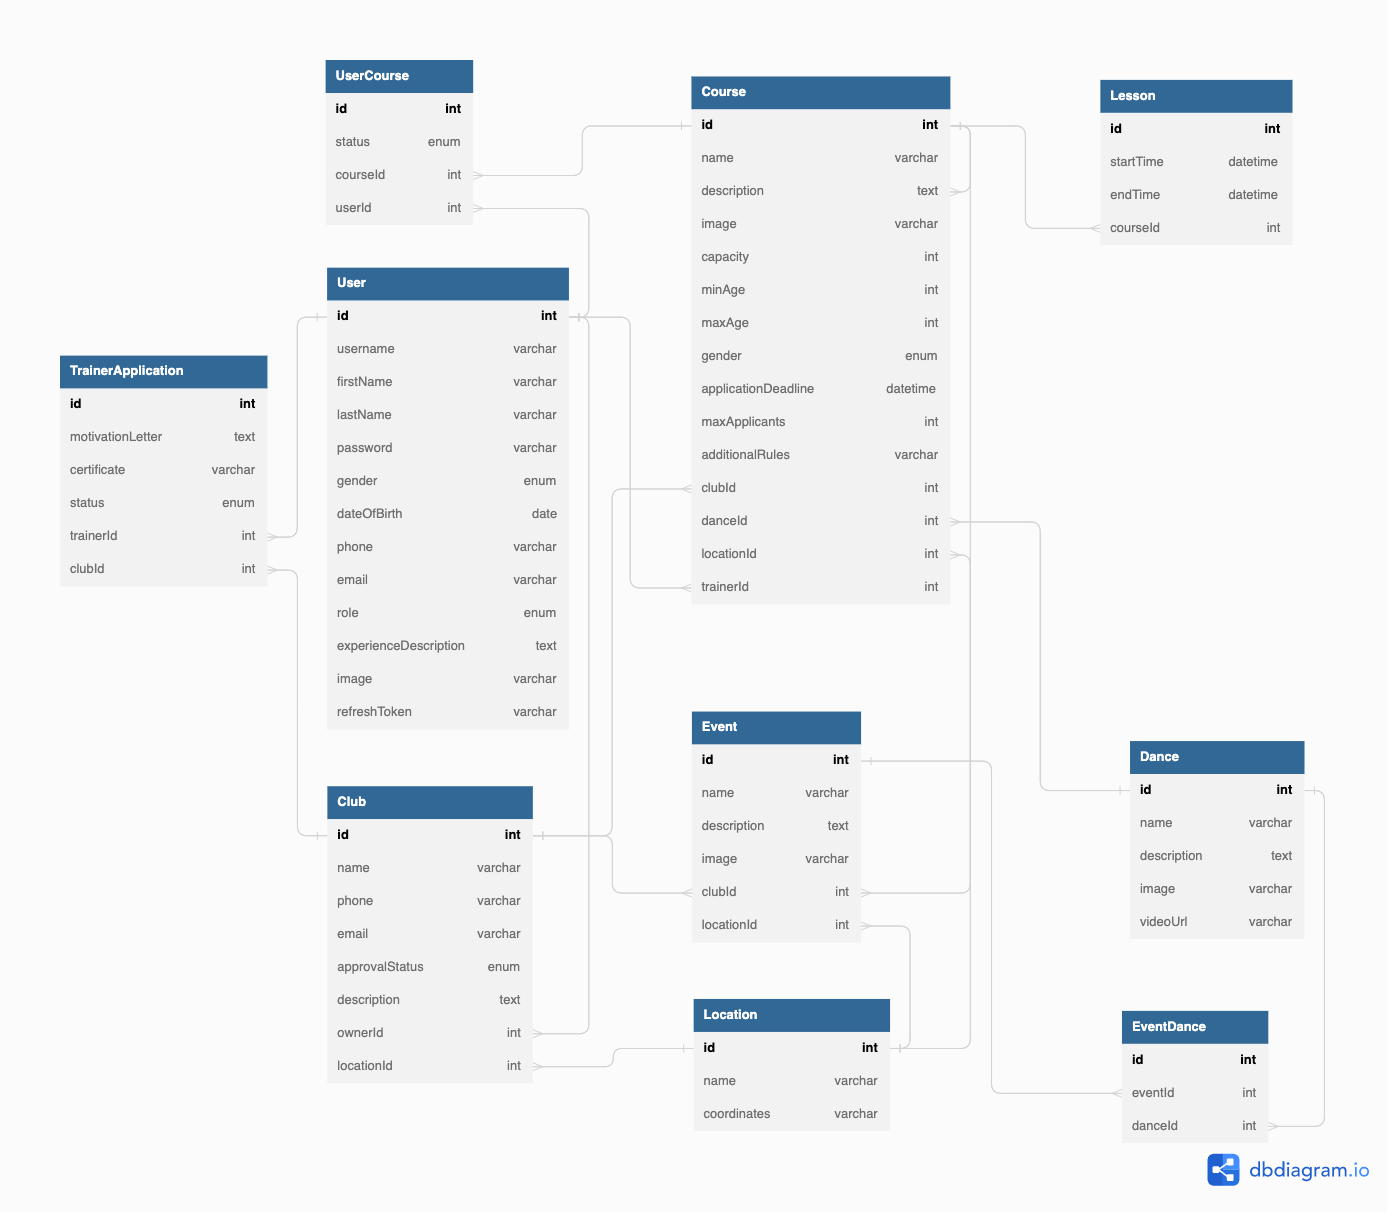
\includegraphics[scale=0.3]{slike/base_diagram.png}
			\centering
			\caption{Relacijski dijagram baze podataka.}
			\label{fig:promjen}
			\end{figure}
			
			\eject
			
			
		\section{Dijagram razreda}
		
			\textit{Na slikama su prikazani razredi koji pripadaju serverskoj strani aplikacije - konkretno modelima i 
			sučeljima koje oni nasljeđuju. Controlleri nisu definirani kao klase nego samoo sadrže funkcije za upravljanje stoga nisu 
			prikazani na klasnom dijagramu.
			Svi modeli nasljeđuju klasu Model. Model razredi preslikavaju strukturu baze podataka u aplikaciji
			Zbog lakše organizacije, dijagram je podijeljen u tri skupine, razredi su podijeljeni logički po dijelovima koji međusobno čine 
			logičku cjelinu ili nasljeđuju i implementiraju zajedničke enumeracuje ili sučelja.
			Iz naziva i tipova atributa u razredima moze se zaključiti vrsta ovisnosti među različitim razredima. }\\
			
			% \textit{Prilikom prve predaje projekta, potrebno je priložiti potpuno razrađen dijagram razreda vezan uz 
			% \textbf{generičku funkcionalnost} sustava. Ostale funkcionalnosti trebaju biti idejno razrađene u dijagramu 
			% sa sljedećim komponentama: nazivi razreda, nazivi metoda i vrste pristupa metodama (npr. javni, zaštićeni), 
			% nazivi atributa razreda, veze i odnosi između razreda.}\\
			\textit{Dijagram koji slijedi prikazuje model Korisnika i Lokacije koji su implementirani u aplikaciji te 
			model TecajModel koji još nije implemetirann te je sklon promjenama. Postoji mogućnost dodavanja novih metoda tijkom implementacije.
			Model User implementira sučelje IUser koji definira njegove atribute i koristi enumeraciju Role i Gender. Role definira ulogu korisnika, a
			Gender spol korisnika. Model Tecaj implementira sučelje ITecaj i korisni enumeraciju Gendr za definiranje spola kojem je tečaj namijenjen.
			}\\
			\begin{figure}[H]
				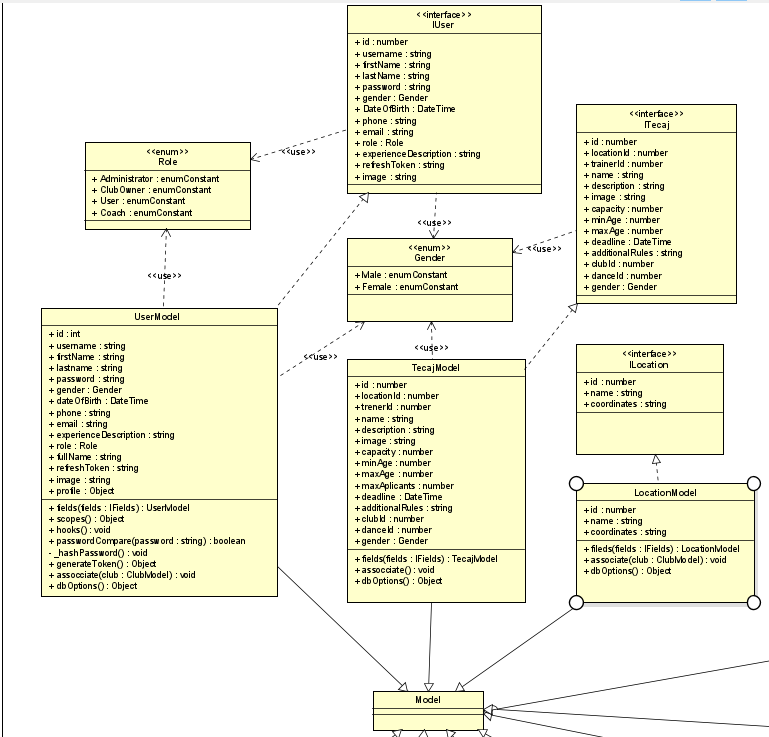
\includegraphics[scale=1.0]{slike/class1.png}
				\centering
				\caption{Dio klasnog dijagrama vezan uz modele User, Tecaj i Location.}
				\label{fig:class1}
			\end{figure}
		% 	\textbf{\textit{dio 2. revizije}}\\			
			
			\textit{Dijagram koji slijedi prikazuje model Kluba koji je implementiran u aplikaciji te modele TrainerApplication i KorisnikTecaj
			koji još nisu implemetirani te su skloni promjenama. Postoji mogućnost dodavanja novih metoda tijkom implementacije.
			Model Klub implemetnira sučelje IKlub koji definira njegove atribute te korisni enumeraciju ApprovalStatus koja opisuje je li 
			administrator prihvatio tog kluba u sustavu ili ne. Klasa HttpError implementira sučelje IHttpError kojom lovimo moguće iznimke 
			nastale u kodu.}\\
			\begin{figure}[H]
				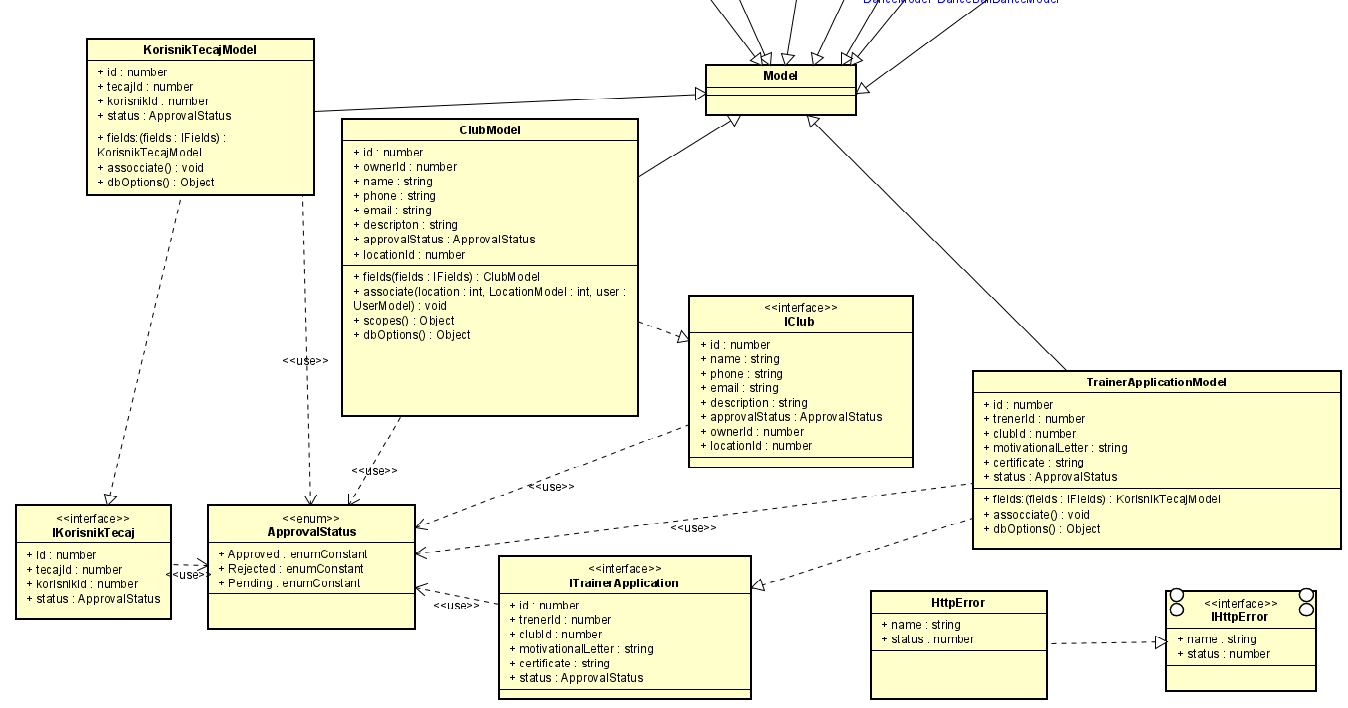
\includegraphics[scale=0.7]{slike/class2.png}
				\centering
				\caption{Dio klasnog dijagrama vezan uz modele Club, TrainerApplication i Korisniktecaj.}
				\label{fig:class1}
			\end{figure}

			\textit{Dijagram koji slijedi priakzuje okvirno stanje modela zato što oni još nisu implementirani. Popisane metode su 
			ugrubo navedene i sklone su promjenama. Postoji mogućnost dodavanja novih metoda tijekom implementacije.}\\
			\begin{figure}[H]
				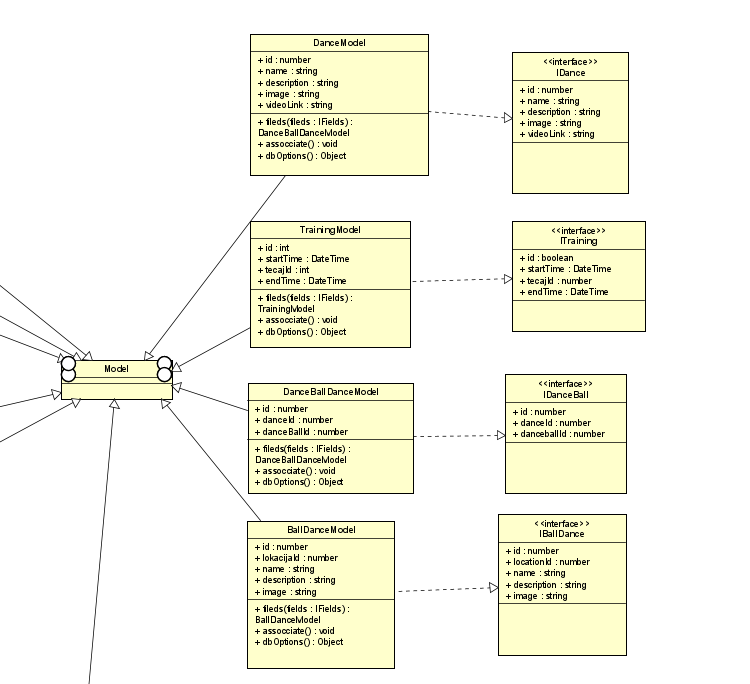
\includegraphics[scale=1.0]{slike/class3.png}
				\centering
				\caption{Dio klasnog dijagrama vezan uz modele Dance, DanceBall i Training.}
				\label{fig:class1}
			\end{figure}

		% 	\textit{Prilikom druge predaje projekta dijagram razreda i opisi moraju odgovarati stvarnom stanju implementacije}
			
			
			
			% \eject
		
		% \section{Dijagram stanja}
			
			
		% 	\textbf{\textit{dio 2. revizije}}\\
			
		% 	\textit{Potrebno je priložiti dijagram stanja i opisati ga. Dovoljan je jedan dijagram stanja koji prikazuje \textbf{značajan dio funkcionalnosti} sustava. Na primjer, stanja korisničkog sučelja i tijek korištenja neke ključne funkcionalnosti jesu značajan dio sustava, a registracija i prijava nisu. }
			
			
		% 	\eject 
		
		% \section{Dijagram aktivnosti}
			
		% 	\textbf{\textit{dio 2. revizije}}\\
			
		% 	 \textit{Potrebno je priložiti dijagram aktivnosti s pripadajućim opisom. Dijagram aktivnosti treba prikazivati značajan dio sustava.}
			
		% 	\eject
		% \section{Dijagram komponenti}
		
		% 	\textbf{\textit{dio 2. revizije}}\\
		
		% 	 \textit{Potrebno je priložiti dijagram komponenti s pripadajućim opisom. Dijagram komponenti treba prikazivati strukturu cijele aplikacije.}
	\chapter{Implementacija i korisničko sučelje}
		
		
		\section{Korištene tehnologije i alati}
		
			\textbf{\textit{dio 2. revizije}}
			
\noindent Komunikacija u timu realizirana je korištenjem aplikacije Slack\footnote{\url{https://slack.com/}} koja omogućuje jednostavnu i veoma organiziranu komunikaciju kroz „channel“ i „therad“ mogućnosti komuniciranja. Za izradu UML dijagrama korišten je alat Astah UML\footnote{\url{https://astah.net/products/astah-uml/}}, a kao sustav za upravljanje izvornim kodom Git\footnote{\url{https://git-scm.com/}}. Udaljeni repozitorij projekta dostupan je na web platformi GitLab\footnote{\url{https://about.gitlab.com/}}.

\noindent Kao razvojno okruženje korišten je Visual Studio Code\footnote{\url{https://code.visualstudio.com/}} – integrirano razvojno okruženje (IDE) tvrtke Microsoft\footnote{\url{https://www.microsoft.com/hr-hr/}} koje dolazi sa ugrađenom podrškom za JavaScript\footnote{\url{https://www.javascript.com/}}, TypeScript\footnote{\url{https://www.microsoft.com/hr-hr/}} i Node.js\footnote{\url{https://nodejs.org/en/}} te pruža IntelliSense\footnote{\url{https://code.visualstudio.com/docs/editor/intellisense}} (inteligentno dovršavanje koda obzirom na kontekst), podršku za otklanjanje pogrešaka, refaktoriranje koda, ugrađene naredbe za Git i mnogobrojna proširenja za ostale programske jezike i alate.

\noindent Klijentska strana aplikacije \textit{(frontend)} napisana je koristeći radni okvir Vue.js\footnote{\url{https://vuejs.org/}} zasnovan na JavaScriptu odnosno TypeScriptu (JavaScript s podrškom za tipove) koji pruža učinkoviti razvoj klijentskog sučelja koristeći već dostupne web komponente i predloške.

\noindent Poslužiteljska strana aplikacije \textit{(backend)} napisana je u programskom jeziku TypeScript koristeći radni okvir Express\footnote{\url{https://expressjs.com/}} koji pojednostavljuje proces izgradnje i razvoja web aplikacija koristeći Node.js. Express pruža funkcionalnosti posredničke arhitekture \textit{(middleware)} i usmjeravanja, jedan je od najpopularnijih okvira za Node.js te se široko koristi za izgradnju malih i velikih web aplikacija. Također, korištena je i ORM \textit{(Object-Relational Mapping)} bilblioteka Sequlize\footnote{\url{https://sequelize.org/}} koja omogućuje interakciju s relacijskim bazama podataka koristeći objektno orijentiranu sintaksu, umjesto izravnih SQL upita.

\noindent Jednostavno pokretanje, konfiguraciju i puštanje u pogon te neovisnost o računalu na kojem se kod izvršava omogućava korištenje platforme Docker\footnote{\url{https://www.docker.com/}}. Kroz tri Docker kontejnera pokriveni su svi ključni dijelovi/slojevi aplikacije – klijent, poslužitelj i PostgreSQL\footnote{\url{https://www.postgresql.org/}} baza podataka te su osigurane točne verzije svih vanjskih biblioteka i alata.
			
			
			\eject 
		
	
		\section{Ispitivanje programskog rješenja}
			
			\textbf{\textit{dio 2. revizije}}\\
			
			 \textit{U ovom poglavlju je potrebno opisati provedbu ispitivanja implementiranih funkcionalnosti na razini komponenti i na razini cijelog sustava s prikazom odabranih ispitnih slučajeva. Studenti trebaju ispitati temeljnu funkcionalnost i rubne uvjete.}
	
			
			\subsection{Ispitivanje komponenti}
			\textit{Potrebno je provesti ispitivanje jedinica (engl. unit testing) nad razredima koji implementiraju temeljne funkcionalnosti. Razraditi \textbf{minimalno 6 ispitnih slučajeva} u kojima će se ispitati redovni slučajevi, rubni uvjeti te izazivanje pogreške (engl. exception throwing). Poželjno je stvoriti i ispitni slučaj koji koristi funkcionalnosti koje nisu implementirane. Potrebno je priložiti izvorni kôd svih ispitnih slučajeva te prikaz rezultata izvođenja ispita u razvojnom okruženju (prolaz/pad ispita). }
			
			
			
			\subsection{Ispitivanje sustava}
			
			 \textit{Potrebno je provesti i opisati ispitivanje sustava koristeći radni okvir Selenium\footnote{\url{https://www.seleniumhq.org/}}. Razraditi \textbf{minimalno 4 ispitna slučaja} u kojima će se ispitati redovni slučajevi, rubni uvjeti te poziv funkcionalnosti koja nije implementirana/izaziva pogrešku kako bi se vidjelo na koji način sustav reagira kada nešto nije u potpunosti ostvareno. Ispitni slučaj se treba sastojati od ulaza (npr. korisničko ime i lozinka), očekivanog izlaza ili rezultata, koraka ispitivanja i dobivenog izlaza ili rezultata.\\ }
			 
			 \textit{Izradu ispitnih slučajeva pomoću radnog okvira Selenium moguće je provesti pomoću jednog od sljedeća dva alata:}
			 \begin{itemize}
			 	\item \textit{dodatak za preglednik \textbf{Selenium IDE} - snimanje korisnikovih akcija radi automatskog ponavljanja ispita	}
			 	\item \textit{\textbf{Selenium WebDriver} - podrška za pisanje ispita u jezicima Java, C\#, PHP koristeći posebno programsko sučelje.}
			 \end{itemize}
		 	\textit{Detalji o korištenju alata Selenium bit će prikazani na posebnom predavanju tijekom semestra.}
			
			\eject 
		
		
		\section{Dijagram razmještaja}
			
			\textbf{\textit{dio 2. revizije}}
			
			 \textit{Potrebno je umetnuti \textbf{specifikacijski} dijagram razmještaja i opisati ga. Moguće je umjesto specifikacijskog dijagrama razmještaja umetnuti dijagram razmještaja instanci, pod uvjetom da taj dijagram bolje opisuje neki važniji dio sustava.}
			
			\eject 
		
		\section{Upute za puštanje u pogon}
		
			\textbf{\textit{dio 2. revizije}}\\
		
			 \textit{U ovom poglavlju potrebno je dati upute za puštanje u pogon (engl. deployment) ostvarene aplikacije. Na primjer, za web aplikacije, opisati postupak kojim se od izvornog kôda dolazi do potpuno postavljene baze podataka i poslužitelja koji odgovara na upite korisnika. Za mobilnu aplikaciju, postupak kojim se aplikacija izgradi, te postavi na neku od trgovina. Za stolnu (engl. desktop) aplikaciju, postupak kojim se aplikacija instalira na računalo. Ukoliko mobilne i stolne aplikacije komuniciraju s poslužiteljem i/ili bazom podataka, opisati i postupak njihovog postavljanja. Pri izradi uputa preporučuje se \textbf{naglasiti korake instalacije uporabom natuknica} te koristiti što je više moguće \textbf{slike ekrana} (engl. screenshots) kako bi upute bile jasne i jednostavne za slijediti.}
			
			
			 \textit{Dovršenu aplikaciju potrebno je pokrenuti na javno dostupnom poslužitelju. Studentima se preporuča korištenje neke od sljedećih besplatnih usluga: \href{https://aws.amazon.com/}{Amazon AWS}, \href{https://azure.microsoft.com/en-us/}{Microsoft Azure} ili \href{https://www.heroku.com/}{Heroku}. Mobilne aplikacije trebaju biti objavljene na F-Droid, Google Play ili Amazon App trgovini.}
			
			
			\eject 
	\chapter{Zaključak i budući rad}
		
		\textbf{\textit{dio 2. revizije}}\\
		
		 \textit{U ovom poglavlju potrebno je napisati osvrt na vrijeme izrade projektnog zadatka, koji su tehnički izazovi prepoznati, jesu li riješeni ili kako bi mogli biti riješeni, koja su znanja stečena pri izradi projekta, koja bi znanja bila posebno potrebna za brže i kvalitetnije ostvarenje projekta i koje bi bile perspektive za nastavak rada u projektnoj grupi.}
		
		 \textit{Potrebno je točno popisati funkcionalnosti koje nisu implementirane u ostvarenoj aplikaciji.}
		
		\eject 
	\chapter*{Popis literature}
		\addcontentsline{toc}{chapter}{Popis literature}
	 	
 		\textbf{\textit{Kontinuirano osvježavanje}}
	
		\textit{Popisati sve reference i literaturu koja je pomogla pri ostvarivanju projekta.}
		
		
		\begin{enumerate}
			
			
			\item  Programsko inženjerstvo, FER ZEMRIS, \url{http://www.fer.hr/predmet/proinz}
			
			\item  I. Sommerville, "Software engineering", 8th ed, Addison Wesley, 2007.
			
			\item  T.C.Lethbridge, R.Langaniere, "Object-Oriented Software Engineering", 2nd ed. McGraw-Hill, 2005.
			
			\item  I. Marsic, Software engineering book``, Department of Electrical and Computer Engineering, Rutgers University, \url{http://www.ece.rutgers.edu/~marsic/books/SE}
			
			\item  The Unified Modeling Language, \url{https://www.uml-diagrams.org/}
			
			\item  Astah Community, \url{http://astah.net/editions/uml-new}
		\end{enumerate}
		
		 
	
	
	\begingroup
	\renewcommand*\listfigurename{Indeks slika i dijagrama}
	%\renewcommand*\listtablename{Indeks tablica}
	%\let\clearpage\relax
	\listoffigures
	%\vspace{10mm}
	%\listoftables
	\endgroup
	\addcontentsline{toc}{chapter}{Indeks slika i dijagrama}


	
	\eject 
		
	\chapter*{Dodatak: Prikaz aktivnosti grupe}
		\addcontentsline{toc}{chapter}{Dodatak: Prikaz aktivnosti grupe}
		
		\section*{Dnevnik sastajanja}
		
		\textbf{\textit{Kontinuirano osvježavanje}}\\
		
		 \textit{U ovom dijelu potrebno je redovito osvježavati dnevnik sastajanja prema predlošku.}
		
		\begin{packed_enum}
			\item  sastanak
			
			\item[] \begin{packed_item}
				\item Datum: 14.10.2022 
				\item Prisustvovali: Mateja Golec, Luka Nola, Nina Đurić, Lara Đaković, Lucija Domić, Ana Vrabec, Karlo Boroš
				\item Teme sastanka: 
				\begin{packed_item}
					\item  upoznavanje
					\item  dogovor oko korištenih tehnologija
					\item  dogovor načina komunikacije
				\end{packed_item}
			\end{packed_item}
			

			\item  sastanak
			
			\item[] \begin{packed_item}
				\item Datum: 20.10.2022 
				\item Prisustvovali: Mateja Golec, Luka Nola, Nina Đurić, Lara Đaković, Lucija Domić, demonstrator, asistent
				\item Teme sastanka:
				\begin{packed_item}
					\item  sastnak s asistentom i demonstratorom
					\item  dogovor funkcionalnosti i rješavanje osnovnih dilema
					\item  dogovor oko korištenih tehnologija
					\item  analiza zadatka
				\end{packed_item}
			\end{packed_item}
			
			\item  sastanak
			\item[] \begin{packed_item}
				\item Datum:  24.10.2022.
				\item Prisustvovali: Mateja Golec, Luka Nola, Nina Đurić, Lara Đaković, Lucija Domić, Ana Vrabec, Karlo Boroš
				\item Teme sastanka:
				\begin{packed_item}
					\item  dogovor oko pisanja dokumentacije i podjele poslova u početnoj fazi
				\end{packed_item}
			\end{packed_item}
			
			\item  sastanak
			\item[] \begin{packed_item}
				\item Datum:  25.10.2022.
				\item Prisustvovali: Luka Nola, Lara Đaković
				\item Teme sastanka:
				\begin{packed_item}
					\item  izrada ER dijagrama baze podataka
				\end{packed_item}
			\end{packed_item}

			\item  sastanak
			\item[] \begin{packed_item}
				\item Datum: 25.10.2022.
				\item Prisustvovali: Mateja Golec, Luka Nola, Nina Đurić, Lara Đaković, Lucija Domić, Ana Vrabec, Karlo boroš
				\item Teme sastanka:
				\begin{packed_item}
					\item  definiranje obrazaca uporabe
					\item  definiranje funkcionalnih zahtjeva
					\item  raspodjela poslova oko izrade obrazaca uporabe, funkcionalnih zahtjeva i opisa zadatka
				\end{packed_item}
			\end{packed_item}

			\item  sastanak
			\item[] \begin{packed_item}
				\item Datum: 27.10.2022.
				\item Prisustvovali: Mateja Golec, Nina Đurić, Lara Đaković, Luka Nola, asistent
				\item Teme sastanka:
				\begin{packed_item}
					\item  pregled funkcionalnih zahtjeva
					\item  pregled obrazaca uporabe
					\item  pregled opisa
					\item  razješavanje dilema za ER dijagram baze podataka
				\end{packed_item}
			\end{packed_item}

			\item  sastanak
			\item[] \begin{packed_item}
				\item Datum: 31.10.2022.
				\item Prisustvovali: Mateja Golec, Nina Đurić, Lara Đaković, Lucija Domić, Ana Vrabec, Karlo Boroš
				\item Teme sastanka:
				\begin{packed_item}
					\item  pregled obrazaca uporabe
					\item  upoznavanje sa latexom
					\item  dogovor za crtanje dijagrama obrazaca uporabe
				\end{packed_item}
			\end{packed_item}

			\item  sastanak
			\item[] \begin{packed_item}
				\item Datum: 4.11.2022.
				\item Prisustvovali: Mateja Golec, Luka Nola, Nina Đurić, Lara Đaković, Lucija Domić, Ana Vrabec, Karlo Boroš
				\item Teme sastanka:
				\begin{packed_item}
					\item  objašnjavanje radnog okruženja i pokretatanje stranice
					\item  definiranje sekvencijskih dijagrama
					\item  raspodjela poslova oko baze podataka i sekvencijskih dijagrama
				\end{packed_item}
			\end{packed_item}

			\item  sastanak
			\item[] \begin{packed_item}
				\item Datum: 9.11.2022.
				\item Prisustvovali: Mateja Golec, Luka Nola, Nina Đurić, Lara Đaković, Lucija Domić, Ana Vrabec, Karlo Boroš
				\item Teme sastanka:
				\begin{packed_item}
					\item  dogovor oko opisa arhitekture
					\item  raspodjela posla i dogovor oko dijagrama razreda
					\item  raspodjela posla i dogovor za autentikaciju i autorizaciju
				\end{packed_item}
			\end{packed_item}

			\item  sastanak
			\item[] \begin{packed_item}
				\item Datum: 10.11.2022.
				\item Prisustvovali: Mateja Golec, Luka Nola, Nina Đurić, Lucija Domić, Ana Vrabec, asistent
				\item Teme sastanka:
				\begin{packed_item}
					\item  pregled dokumentacije
					\item  razrješavanje pitanja u vezi baze,  autorizacije i klasnih dijagrama
				\end{packed_item}
			\end{packed_item}

			\item  sastanak
			\item[] \begin{packed_item}
				\item Datum: 14.11.2022.
				\item Prisustvovali: Mateja Golec, Luka Nola, Nina Đurić, Lara Đaković, Lucija Domić, Ana Vrabec, Karlo Boroš
				\item Teme sastanka:
				\begin{packed_item}
					\item  pregled rada aplikacije
					\item  dovršavanje klasnih dijagrama
				\end{packed_item}
			\end{packed_item}
		
			\item  sastanak
			\item[] \begin{packed_item}
				\item Datum: u ovom formatu: 16.11.2022.
				\item Prisustvovali: Mateja Golec, Luka Nola, Nina Đurić, Lara Đaković, Lucija Domić, Ana Vrabec, Karlo Boroš
				\item Teme sastanka:
				\begin{packed_item}
				    \item  provjera rada stranice
					\item  revizija obavljenog posla
					\item  dogovor oko potrebnih izmjena
				\end{packed_item}
			\end{packed_item}

		\end{packed_enum}
		
		\eject
		\section*{Tablica aktivnosti}
		
			\textbf{\textit{Kontinuirano osvježavanje}}\\
			
			 \textit{Napomena: Doprinose u aktivnostima treba navesti u satima po članovima grupe po aktivnosti.}

			\begin{longtblr}[
					label=none,
				]{
					vlines,hlines,
					width = \textwidth,
					colspec={X[7, l]X[1, c]X[1, c]X[1, c]X[1, c]X[1, c]X[1, c]X[1, c]}, 
					vline{1} = {1}{text=\clap{}},
					hline{1} = {1}{text=\clap{}},
					rowhead = 1,
				} 
				\multicolumn{1}{c|}{} & \multicolumn{1}{c|}{\rotatebox{90}{\textbf{Mateja Golec}}} & \multicolumn{1}{c|}{\rotatebox{90}{\textbf{Karlo Boroš }}} & \multicolumn{1}{c|}{\rotatebox{90}{\textbf{Lucija Domić}}} & \multicolumn{1}{c|}{\rotatebox{90}{\textbf{Lara Đaković}}} & \multicolumn{1}{c|}{\rotatebox{90}{\textbf{Nina Đurić}}} & \multicolumn{1}{c|}{\rotatebox{90}{\textbf{Luka Nola}}} & \multicolumn{1}{c|}{\rotatebox{90}{\textbf{Ana Vrabec}}}  \\
				Upravljanje projektom 		& 15h & 13h &  & 14h & 13h &  & \\ 
				Opis projektnog zadatka 	&  &  &  &  & 6h &  & \\ 
				
				Funkcionalni zahtjevi       &3h  &  &  &  &  &  &  \\ 
				Opis pojedinih obrazaca 	&  & 5h &  & 7h &  &  &  \\ 
				Dijagram obrazaca 			&  & 3h &  & 4h &  &  &  \\ 
				Sekvencijski dijagrami 		&4h  &  &  &  & 2h &  &  \\  
				Opis ostalih zahtjeva 		&  &  &  &  &  &  &  \\ 

				Arhitektura i dizajn sustava	 &3h  &  &  &  &  &  &  \\ 
				Baza podataka				&  & 5h &  & 5h &  &  &   \\ 
				Dijagram razreda 			&  &  &  & 5h & 2h &  &   \\  
				Dijagram stanja				&  &  &  &  &  &  &  \\ 
				Dijagram aktivnosti 		&  &  &  &  &  &  &  \\ 
				Dijagram komponenti			&  &  &  &  &  &  &  \\ 
				Korištene tehnologije i alati 		&  &  &  &  &  &  &  \\ 
				Ispitivanje programskog rješenja 	&  &  &  &  &  &  &  \\ 
				Dijagram razmještaja			&  &  &  &  &  &  &  \\ 
				Upute za puštanje u pogon 		&  &  &  &  &  &  &  \\  
				Dnevnik sastajanja 			&  &  &  & 2h &  &  &  \\ 
				Zaključak i budući rad 		&  &  &  &  &  &  &  \\  
				Popis literature 			&  &  &  &  &  &  &  \\  
				&  &  &  &  &  &  &  \\ \hline 
				\textit{Dodatne stavke kako ste podijelili izradu aplikacije} 			&  &  &  &  &  &  &  \\ 
				\textit{izrada početne stranice} 				&  &  &  &  &  &  &  \\  
				\textit{izrada baze podataka} 		 			&  &  &  & 4h &  &  & \\  
				\textit{Autorizacija i autentikacija - backend}	&  & 5h &  &  &  &  &  \\
				\textit{spajanje s bazom podataka} 							&  &  &  &  &  &  &  \\ 
				\textit{back end} 							&  &  &  &  &  &  &  \\  
				 							&  &  &  &  &  &  &\\ 
			\end{longtblr}
					
					
		\eject
		\section*{Dijagrami pregleda promjena}
		
		\textbf{\textit{dio 2. revizije}}\\
		
		\textit{Prenijeti dijagram pregleda promjena nad datotekama projekta. Potrebno je na kraju projekta generirane grafove s gitlaba prenijeti u ovo poglavlje dokumentacije. Dijagrami za vlastiti projekt se mogu preuzeti s gitlab.com stranice, u izborniku Repository, pritiskom na stavku Contributors.}
		
	


\end{document} %naredbe i tekst nakon ove naredbe ne ulaze u izgrađen dokument 


